\section{Résultats sur un échantillon de mèmes}
\label{sec:results-memes}

Nous présentons maintenant les résultats obtenus grâce à notre dispositifs d'analyse sur un échantillon d'une dizaine de mèmes. La typologie de mèmes identifiées précédemment (voir fig. \ref{fig:typologie-memes}) a servi de point de départ pour cette sélection. Une recherche mêlant littérature scientifique et secondaire (journaux, blogs, encyclopédies en ligne, sites ressources) ainsi que notre propre expérience du web chinois nous a permis de définir un panel de mèmes observables dans par notre corpus (voir annexe \ref{sec:fullmemes}). 

\begin{table}[h!]
  \begin{tabulary}{\textwidth}{c|C}

    \textbf{Nom} &
    \textbf{Description}\\
    \hline \\[-1.5ex]
    \textit{Sextape} &
    Un scandale d{\textquoteright}adultère concernant un homme politique
    dans la ville de Chongqing dans le centre de la Chine.\\[2ex]

    \textit{The Voice} &
    La première saison d{\textquoteright}une émission de
    télé-crochet musical en Chine.\\[2ex]

    \textit{Qiegao} &
    Un débat de société sur la condition du peuple Uyghur suivant un
    fait divers autour d{\textquoteright}une rixe lors
    d{\textquoteright}une vente de gâteau.\\[2ex]

    \textit{Dufu} &
    Un mème comique mettant en scène un poète chinois dans des
    situations burlesques.\\[2ex]

    \textit{Biaoge} &
    Un scandale entourant la collection de montres de marques prestigieuses
    d{\textquoteright}un homme politique de la province du Shaanxi \\[2ex]

    \textit{Moyan} &
    L{\textquoteright}attribution du Prix Nobel de littérature \`a
    l{\textquoteright}écrivain chinois Mo Yan\\[2ex]

    \textit{Yuanfang} &
    La reprise d{\textquoteright}une citation d{\textquoteright}une série
    télévisée sous forme humoristique\\[2ex]

    \textit{Ccp} &
    Les débats entourant le 18ème Congrès du Parti Communiste Chinois\\[2ex]

  \end{tabulary}
  \caption{Dénomination et description des mèmes étudiés}
  \label{fig:meme-sample}
\end{table}


Dans un premier temps, nous avons lister différents mèmes et événements web de l{\textquoteright}année 2012 sur \textit{Sina Weibo} (voir annexe \ref{fig:memelist}). Ensuite, nous avons chercher à constituer un ensemble cohérent montrant la diversité des contenus pour l'étude (voir \ref{fig:meme-sample})Les différentes sources consultées proposent des définitions très différentes de l'objet mème. De nombreux sites Web effectuent a posteriori une revue des faits et contenus qu'ils considèrent comme les plus marquants de l'Internet chinois en 2012. Micro-historiographie du web, ce type de classification affirmant l'importance supposée des événements web reflète néanmoins plutôt l'orientation éditoriale de l'auteur ou du média qu'une réalité historique. Sur les sites anglophones, les contenus marquant du web social chinois en 2012 ont tous un caractère politique et polémique. Les listes les plus largement reprises ont été constituées par des sites généralistes comme \textit{Global Voices}\footnote{Global Voices, \url{http://globalvoicesonline.org/2012/12/07/top-10-chinese-internet-memes-of-2012/}, consulté le 22 Avril 2014 à 12:10} ou le \textit{Wall Street Journal}\footnote{ Wall Street Journal http://blogs.wsj.com/chinarealtime/2012/12/19/the-top-10-chinese-internet-memes-of-2012/,consulté le 22 Avril 2014 à 12:10}. Largement repris par des professionnels, journalistes ou blogueurs, ces supports influents proposent une sélection de mèmes tournés vers la satire politique. Plusieurs sont directement liés à des campagnes de soutien pro-démocratie dont la diffusion dans le paysage médiatique contrôlée de la Chine reste extrêmement marginale, voire souterraine. D'autres actualités fortes ont donné lieu à des débats d'ampleur nationale. Faits divers et scandales éclaboussant des hommes politiques chinois impliquent très largement l'audience des réseaux sociaux qui commentent abondamment sur la situation politique alarmante et la corruption des gouvernements locaux. 

L'affaire Yang Dacai, baptisé ``Brother Watch''(\textit{biaoge}, \zh{表哥}), a notamment fait coulé beaucoup d'encre numérique sur les écrans chinois. En Août 2012, Yang Dacai, directeur du Bureau de Supervision de la Sécurité Routière de la province du Shanxi, se rend sur les lieux d'un accident de bus ayant fait 36 morts. Une photo diffusée sur Internet le montre discutant avec un policier, arborant un grand sourire. Agacé par cet excès d'incivilité, les internautes commencent à faire des recherches à son sujet et remarquent que l'officiel chinois arbore à chaque apparition une montre différente, toutes de marques prestigieuses. Il est rapidement surnommé \textit{le frère aux montres} (\textit{biaoge}). Les collections de photos de ses différentes montres de luxe circulent comme autant de preuves flagrantes de sa corruption. Quelques jours plus tard, Yang Dacai est démis de ces fonctions. Il sera par la suite jugé et condamné pour corruption, assorti d'une peine de 12 ans de prison (voir les détails dans l'annexe \ref{sec:biaoge}). 

\begin{figure}[htbp]
    \hspace{\fill}%
    \subfloat[La photo montrant Yang Dacai ``frère montre'' souriant sur la scène du crash.]{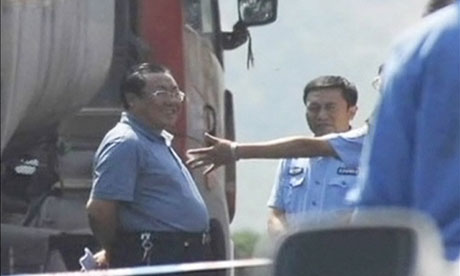
\includegraphics[scale=.56]{figures/annexes/biaoge/Yang-Dacai-smiling.jpg}}
    \hspace{\fill}%
    \subfloat[Un an plus tard, Yang Dacai plaide coupable pour corruption lors de son jugement]{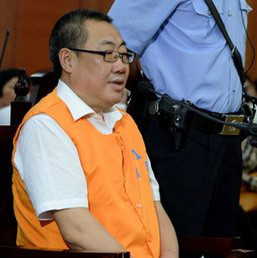
\includegraphics[scale=.8]{figures/annexes/biaoge/biaoge-jailed-thumb.jpg}}
    \hspace{\fill}%
    \caption{ 
      Illustrations du mème \textit{biaoge} d'après le Guardian \url{http://www.theguardian.com/world/2013/sep/05/china-brother-wristwatch-yang-dacai-sentenced}, consulté le 7 Juillet 2014 à 12:11. et la BBC \url{http://www.bbc.com/news/world-asia-china-23956170}, consulté le 7 Juillet 2014 à 12:23.
    }
\end{figure}

Parmi les autres affaires remarquables en 2012 se trouve celle de la \textit{sextape} montrant Lei Zhengfu, le secrétaire du Parti dans le district de Beibei à Chongqing dans le plus simple appareil en compagnie d'une de ses maîtresses. A peine 63h après la publication de cette vidéo avec le titre \textit{``Lei, the secretary who accepts sex bribes''}, Lei fut mis à pied de ses fonctions politiques. La rapidité de cette action est alors présentée publiquement comme le résultat du nouveau programme de \textit{surveillance du réseau par l'opinion publique}\footnote{http://www.chinanews.com/gn/2012/11-24/4354915.shtml, consulté le 9 Juillet à 12:41}. Cette vidéo qui avait été tournée 4 ans auparavant été utilisée depuis plusieurs années par un promoteur immobilier de la ville de Chongqing pour faire chanter Lei Zhengfu (voir annexe \ref{sec:sextape}). 

Un dernier fait divers n'impliquant cette fois pas des hommes politiques mais des citoyens chinois de l'ethnie ouïghour a également retenue notre attention. Originaire d'Asie centrale et orientale, le peuple ouïghour vit dans la région du Xinjiang, en Chine occidentale. Turcophones et majoritairement musulmans, les us et coutumes de ce peuple entrent bien souvent en contradiction avec ceux des chinois orientaux. La forte présence militaire chinoise dans la région et le ressenti qui anime les relations entre les peuples chinois et ouïghour conduisent régulièrement à des affrontements. Cette forte tension est également palpable dans les grandes villes de la côte comme Canton, Shanghai ou Pékin où les habitants du Xinjiang ont immigré en masse. La plupart travaillent dans des petits commerces de bouche. Une des spécialités de la région du Xinjiang est un délicieux gâteau à base de riz gluant, de noix et de jujube nommé \textit{qiegao} (\zh{切糕}). Vendu le plus souvent dans la rue, il se coupe difficilement. Son prix est plutôt élevé (jusqu'à 10 euros le kilo). Les vendeurs sont connus pour jouer de cette découpe compliquée comme excuse pour servir de généreuses portions aux clients, parfois plus larges que celles demandées. Une part un peu trop grosse découpée par un des vendeurs a mené à une rixe avec un client chinois fort mécontent. Escaladant en bagarre générale, cette altercation s'est terminé par l'arrivée de la police qui a séparé rapidement les belligérants. Cette histoire fort banale ce serait arrêtée là si les internautes n'avaient pas eu vent du prix de 200 000 RMB (25 000 euros) réclamé par les vendeurs en dédommagement de leur marchandise et des dommages causés (blessures, motos brisées, etc). Parcourant rapidement la toile, cette nouvelle soulève de nombreuses questions des internautes, raillant sur le coût faramineux du gâteau : \textit{``A piece of Xinjiang nut cake about 1.6 square meters in size cost RMB 160,000, which means about RMB 100,000 per square meter. Every 1 square meter of Xinjiang nut cake can buy about 3 square meters of apartment in Beijing.''}\footnote{d'après Off Beat China \url{http://offbeatchina.com/an-unbelievably-expensive-piece-of-xinjiang-nut-cake-and-what-it-tells-about-the-ethnic-policy-in-china}, consulté le 7 Juillet à 13:02}. Entre commentaires racistes, discussions houleuses et blagues de tous bords, ce fait divers du \textit{qiegao} amène à un débat national de plusieurs jours sur la condition des minorités ouïgoures dans les villes chinoises impliquant médias, universitaires et citoyens. 

\begin{figure}[h!]
    \centering
    \subfloat[Une image de l'affrontement avec la police posté par un utilisateur de Sina Weibo]{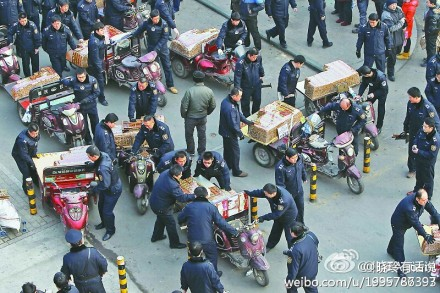
\includegraphics[scale=.65]{figures/annexes/qiegao/1.jpg}}
    \subfloat[Création d'un internaute montrant combien le qiegao est cher]{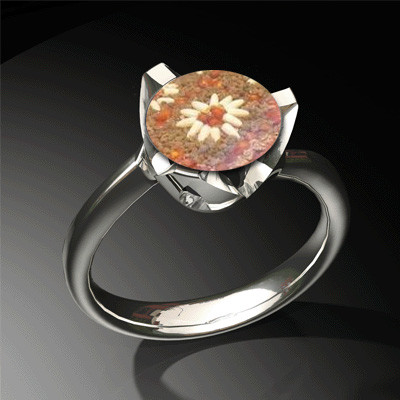
\includegraphics[scale=.66]{figures/annexes/qiegao/2.jpg}}
    \caption{
      Quelques images du mème \textit{qiegao}
    }
\end{figure}

Note étude sur les hashtags a montré que les réseaux sociaux en Chine sont également le lieu de vastes campagnes commerciales. Dans les plus  grands événements du Web en Chine, le site spécialisé \textit{Danwei}\footnote{ Danwei \url{http://www.danwei.com/chinas-hottest-styles-of-2012/} consulté le 22 Avril 2014 à 12:12} note que de nombreuses émissions de télévision ont générées une participation considérable sur Internet également. Ainsi, nous avons choisi pour représenter cette catégorie la version chinoise de l'émission internationalement connue de radio-crochet ``The Voice'' (\zh{中国好声音}, \textit{zhongguo hao shengyin}). Ayant battu en 2012 tous les records d'audience, \textit{The Voice of China} offre un exemple parlant des grandes campagnes trans-médiatiques qui touche \textit{Sina Weibo}.

Si la représentation des réseaux sociaux chinois comme un outil d'expression politique et de domination médiatique est souvent portée par les médias étrangers, les médias chinois dont \textit{Baidu} publient une sélection des mots les plus marquants à chaque fin d'année\footnote{Lire \textit{Les 10 mots de l'Internet en 2012} sur \textit{Baidupedia} \url{http://baike.baidu.com/view/9710412.htm}, consulté le 9 Juillet 2014 à 10:32}. Le mot \textit{mème} ne possède pas de traduction chinoise à proprement parler \citep{Renaud2014}. Ainsi, la sélection de fin d'année se fait la plupart du temps sous la forme d'une liste de ``mots à la mode'' (\zh{流行语}, \textit{liuxingci}). Aucune des campagnes pro-démocratie ou même des ``événements web'' considérés comme marquants par les médias généralistes occidentaux n'est présent dans cette liste. On y retrouve par contre un humour noir et sarcastique, un des traits caractéristiques de l'Internet chinois d'aujourd'hui. Ces expressions humoristiques en disent long sur la société chinoise moderne. \textit{Yalishan da} (\zh{压力山大}) est un homophone du nom chinois d'Alexandre le Grand mais signifie littéralement ``La montagne du stress est grande.''. Ce jeu de mot invoquant la figure mythologique du conquérant témoigne de l'immense pression pour la survie et la réussite qui s'exerce au quotidien sur les jeunes urbains chinois. Ici, le rire caustique qui fait de ce simple jeu de mots un succès sur l'Internet semble agir comme un exutoire dans la compétition sans relâche que réclame la société chinoise moderne. 

Les interrogations sur la réalité quotidienne se poursuivent avec en seconde place du classement des mots de l'Internet en 2012 la question \textit{``Es-tu heureux?''} (\zh{你幸福吗}). Avant de devenir une des citations les plus commentées de l'année 2012, cette question fût posée lors d'une interview sur la première chaîne officielle chinoise \textit{CCTV1} au prix Nobel de littérature chinois Mo Yan. Sa réponse incluant \textit{``avoir une belle maison''} et \textit{``une bonne éducation''} déclencha de longues discussions et débats en ligne sur l'infinie question de la définition du bonheur dans une Chine en plein développement (``\zh{2012年,开发商,你们幸福吗?}''). 

Également, de nouveaux mots ont fait leur apparition comme le très notable \textit{diaosi} (\zh{屌丝}) aujourd'hui largement usité dans le langage commun\footnote{`` a buzzword, referring to a young man born in a humble family, with mediocre appearance and working in a dead-end job'' sur \url{https://en.wikipedia.org/wiki/Diaosi}, consulté le 7 Juillet 2014 à 11:12}. Depuis 2010, ce mot désigne un jeune homme d'origine modeste, célibataire, sans argent ni bien, qui travaille dans un métier sans intérêt ni avenir, souvent derrière un ordinateur. Proche de l'idée de \textit{No Life} en anglais ou de \textit{otaku} en japonais, \textit{diaosi} porte également en lui le mal-être des jeunes générations d'urbains désargentés, face à l'impossibilité de trouver un métier ou une vie familiale plaisante. 

Ces quelques exemples montrent bien les nombreuses discussions sur la condition moderne et la société actuelle en Chine qui animent les internautes chinois. La noirceur de l'humour et le réalisme des débats donne une image plutôt sérieuse voir obséquieuse des réseaux sociaux chinois. Nous devons nous empresser de nuancer ce propos : les photos d'animaux domestiques ou de nourritures y restent avant tout les contenus les plus courants. L'humour peut également être beaucoup plus léger avec des mèmes aux contenus aussi absurdes que comiques. Une série policière très prisée présentant un couple de détectives enquêtant dans la Chine médiévale procura notamment de bonne doses de rire aux spectateurs. Dialogue récurrent de la série, la phrase \textit{``Yuanfang, qu'en penses-tu?''} (\zh{元芳,你怎么看?}) s'est hissée en peu de temps à une célébrité semblable au \textit{``élémentaire''} de Sherlock Holmes au Dr. Watson. Le poète chinois Du Fu de la dynastie Tang a également connu un retour fulgurant sous la forme de peintures détournées le mettant en scène dans des situations improbables : ``Du Fu est vraiment très occupé'' (\zh{杜甫很忙}). 

\begin{figure}[htbp]
    \hspace{\fill}
    \subfloat[Dufu is very busy] {
      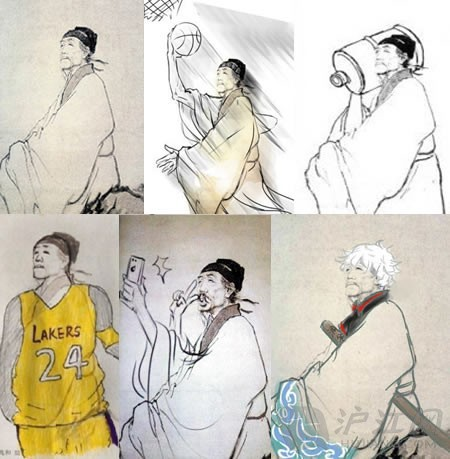
\includegraphics[scale=.5]{figures/annexes/dufu/dufu-busy-2.jpg}
      \label{}
    }
    \hspace{\fill}%
    \subfloat[Yuanfang, qu'en penses-tu?] {
      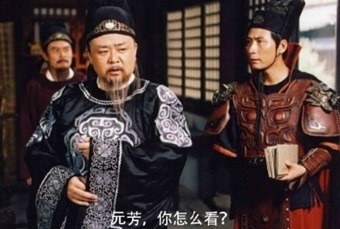
\includegraphics[scale=.9]{figures/annexes/yuanfang/Yuan-Fang-what-do-you-think.jpg}
      \label{}
    }
    \hspace{\fill}%
    \caption{}
    \label{}
\end{figure}


L'échantillon que nous avons choisi d'étudier reflète la diversité de ces contenus (voir la liste \ref{fig:meme-sample}). Ainsi, l'échantillon contient autant des actualités nationales importantes (comme le 18ème Congrès du Parti Communiste Chinois ou l'attribution du prix Nobel de littérature à l'écrivain chinois Mo Yan) que des mèmes comiques et absurdes (``Yuanfang, qu'en penses-tu?'' et ``Du Fu est vraiment très occupé''). Également, nous avons retenu plusieurs faits divers (la sextape de Lei Zhengfu, les montres de \textit{biaoge} ou le gâteau \textit{qiegao} du Xinjiang) et une émission de télévision \textit{The Voice}. Les différents contenus choisis vont nous permettre de mieux comprendre les modèles de diffusion en établissant des comparaisons.

Une présentation plus détaillée de chacun des mèmes choisis est disponible en annexe de cette thèse (Figure \ref{sec:fullmemes}). Pour une meilleure commodité de lecture, un nom a été attribué \`a chacun d'eux afin de pouvoir les évoquer facilement dans la suite de l'étude. A l'aide de l'outil que nous avons développé, nous allons maintenant observer dans le détail la diffusion de chacun de ces mèmes. 

\newpage

\subsection[Structures temporelles]{Structures temporelles}

Dans un premier temps, nous avons choisi de considérer les différentes structures temporelles qui émergent de la diffusion de ces mèmes. La première série de figures ci-dessous (fig. \ref{fig:time-patterns}) représente chronologiquement le volume de messages échangés par heure dans chacun des jeux de données. La période totale couverte par les échantillons est de 3 semaines. La première observation concerne la diminution quotidienne du volume de messages dessinant des pics réguliers. Cette forme spécifique correspond tout simplement \`a la baisse de l{\textquoteright}activité des utilisateurs de \textit{Sina Weibo} pendant la nuit.

Nous voyons également émerger différentes formes représentatives pour chacune des catégories choisies : le fait divers ({\textquotedblleft}breaking news{\textquotedblright}) représenté par le mème \textit{qiegao} débute très nettement avec une augmentation abrupte de la quantité de message postés en très peu de temps (Fig. \ref{fig:time-qiegao}). Atteignant un niveau très élevé quasiment instantanément, ce pic est suivi d{\textquoteright}une retombée rapide de l{\textquoteright}attention quelques jours plus tard.  

A l'inverse, la discussion plus informative autour du procès de l{\textquoteright}homme politique de Chongqing et sa {\textquotedblleft}sextape{\textquotedblright} (Fig. \ref{fig:time-sextape}) croit doucement pour conna\^itre un pic très fort de discussion. L'attention retombe rapidement, consécutivement à la prise en main rapide de cette affaire par le gouvernement et les médias locaux.

L{\textquoteright}émission de télévision \textit{The Voice} est, elle, absolument événementielle. Son graphe montre nettement le rythme clairsemé des émissions, accompagné de très peu de discussions seulement entre chacune d'elles (Fig. \ref{fig:time-voice}). Néanmoins, le volume de messages échangés est nettement plus important que dans les autres cas, avec un pic de plus de 2000 tweets par heure (dans notre corpus) le soir de la première émission, dépassant très largement le volume des trois autres mèmes présentés ici.

\begin{figure}[ht]
    \centering
    \subfloat[sextape]{
      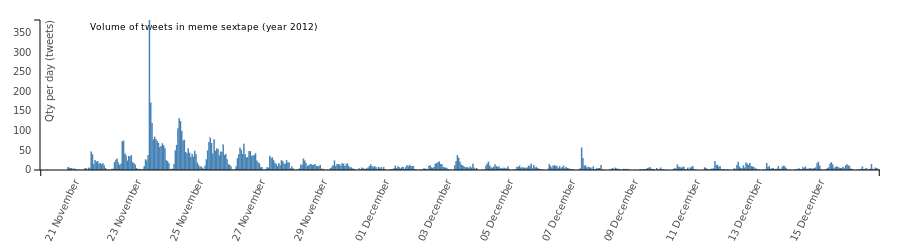
\includegraphics[width=6.0087in,height=1.6697in]{figures/chap4/chapitre4-img1.png}
      \label{fig:time-sextape}
    }
    \newline
    \subfloat[dufu]{
      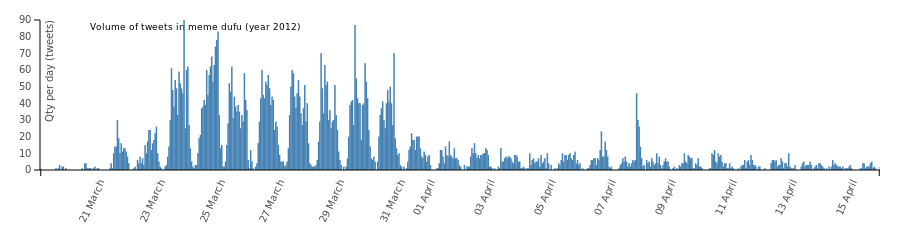
\includegraphics[width=6.0087in,height=1.6697in]{figures/chap4/chapitre4-img2.png}
      \label{fig:time-dufu}
    }
    \newline
    \subfloat[qiegao]{
      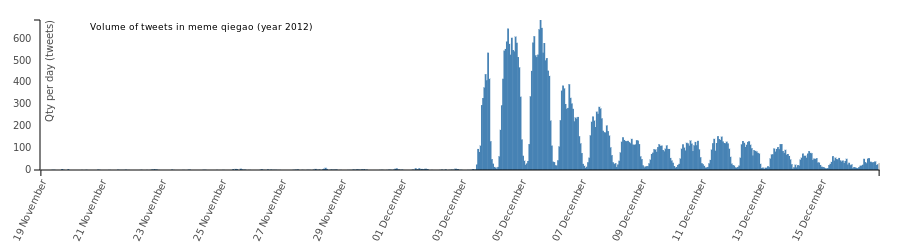
\includegraphics[width=6.0087in,height=1.6697in]{figures/chap4/chapitre4-img3.png}
      \label{fig:time-qiegao}
    }
    \newline
    \subfloat[The Voice]{
      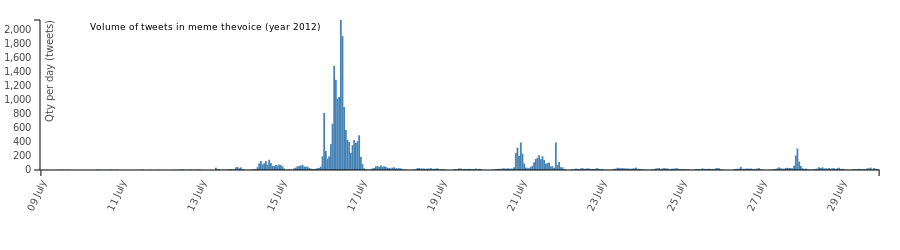
\includegraphics[width=6.0087in,height=1.6697in]{figures/chap4/chapitre4-img4.png}
      \label{fig:time-voice}
    }
    \caption{
      Graphe temporel représentant le volume de messages échangés autour de 4 mèmes sur une durée de 3 semaines 
    }
    \label{fig:time-patterns}
\end{figure}
\clearpage

Le graphe du mème absurdiste \textit{dufu} connaît quant à lui une lente montée d{\textquoteright}attention puis un plateau de plusieurs jours (fig. \ref{fig:time-dufu}). La blague semble durer et même conna\^itre un regain d{\textquoteright}intérêt une semaine plus tard. Elle est ensuite régulièrement mentionnée durant les jours suivants, montrant davantage de persistance que les autres types de contenus.

Proportionnellement, nous constatons que le mème absurdiste est donc celui qui retient le plus l{\textquoteright}attention, le plus longtemps (Fig. \ref{fig:time-dufu}). A l{\textquoteright}inverse la campagne en ligne de \textit{The Voice} n{\textquoteright}est qu{\textquoteright}un artefact de l{\textquoteright}émission (Fig. \ref{fig:time-voice}) mais draine une audience très importante pendant un temps restreint. Le cycle des actualités semble être plus court, arrivant rapidement pour disparaître tout aussi vite.

\begin{figure}[h!]
    \centering
    
  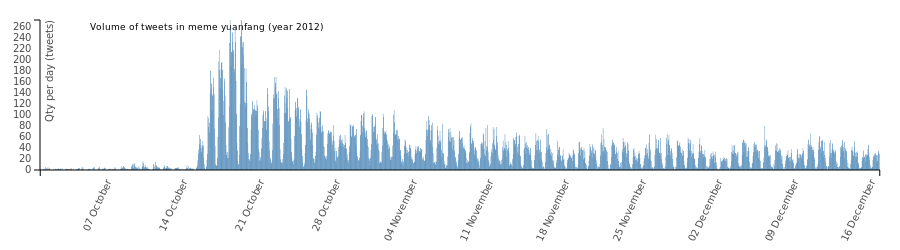
\includegraphics[width=6.0087in,height=1.6697in]{figures/chap4/chapitre4-img5.png}
  \caption{
   Graphe temporel représentant le volume de messages échangés  autour du mème \textit{yuanfang} entre le 7 Octobre et le 16 Décembre 2012.
  }
  \label{fig:time-yuanfang}
\end{figure}

En observant un second contenu comique (\textit{yuanfang}) sur une période beaucoup plus longue de plusieurs mois (ici du 7 Octobre au 16 Décembre 2012) (fig. \ref{fig:time-yuanfang}), nous pouvons vérifier la tendance des mème humoristiques \`a durer dans le temps. \textit{Yuanfang} continue d{\textquoteright}être mentionné très régulièrement même des mois après sa première apparition. 

\begin{figure}[h!]
    \centering
    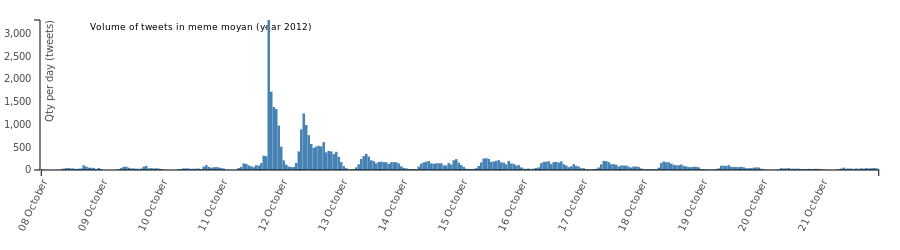
\includegraphics[width=6.0087in,height=1.6697in]{figures/chap4/chapitre4-img6.png}
    \caption{
      Graphe temporel représentant le volume de messages échangés autour du mème \textit{moyan} entre le 8 et le 21 Octobre 2012.
    }
    \label{fig:time-moyan}
\end{figure}

A l{\textquoteright}inverse, les actualités du type {\textquotedblleft}news{\textquotedblright} ont une durée de vie très courte, même lorsqu{\textquoteright}elles sont très débattues. Dans le cas de \textit{moyan}, on voit un très fort volume d{\textquoteright}activité (3000 messages par heure au plus haut) mais une disparition quasi-totale des débats au bout en moins d{\textquoteright}une dizaine de jours (Fig. \ref{fig:time-moyan}).

Les cycles de vie des actualités ou des scandales en ligne sont déjà largement connus et documentés. Cette approche montre néanmoins une nouveauté : la dimension humoristique et absurdiste de certains mèmes leur permet une diffusion à moyen terme.

\subsection[Structures conversationnelles]{Structures conversationnelles}

Les conversations sur Sina Weibo sont faites d{\textquoteright}échanges entre les utilisateurs sous la forme de commentaires, de promotion d{\textquoteright}un message (\textit{zhuanfa} ou \zh{转发} équivalent du {\textquotedblleft}retweet{\textquotedblright} de Twitter) ou de réponse au message. Mises bout à bout, ces différentes interactions forment une large conversation o\`u les utilisateurs interagissent, se parlent, se répondent, discutent en utilisant les différentes fonctionnalités de la plate-forme. En simplifiant ces échanges sous la forme de relations dirigées entre deux utilisateurs (\textit{{\textquotedblleft}A interagit avec B{\textquotedblright}}), nous pouvons reconstituer le réseau dirigé des interactions que nous visualisons ensuite sous la forme d{\textquoteright}un graphe. Dans ce réseau conversationnel, les individus sont symbolisés par des points au sein des communautés notées par différentes couleurs sélectionnées pour leur cohérence et leur visibilité \citep{Lin2013}. La taille des cercles indique leur degré dans le réseau global (total des connections entrantes et sortantes).


\begin{figure}[h!]
    \centering
    \subfloat[Sextape]{
      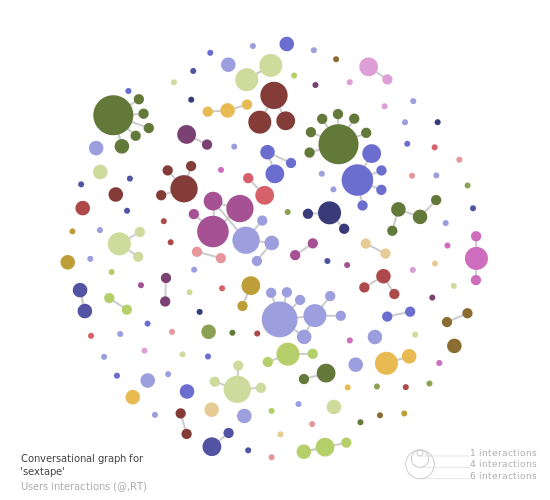
\includegraphics[width=3.0705in,height=2.7913in]{figures/chap4/chapitre4-img7.png}
      \label{fig:users-sextape}
    }
    \subfloat[The Voice]{
      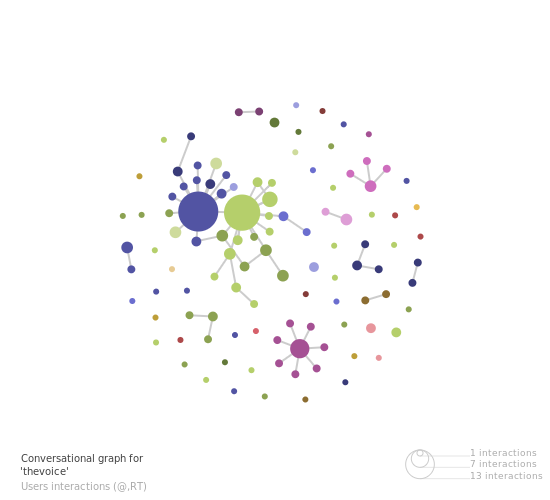
\includegraphics[width=3.0705in,height=2.7913in]{figures/chap4/chapitre4-img8.png}
      \label{fig:users-voice}
    }
    \newline
    \subfloat[Qiegao]{
      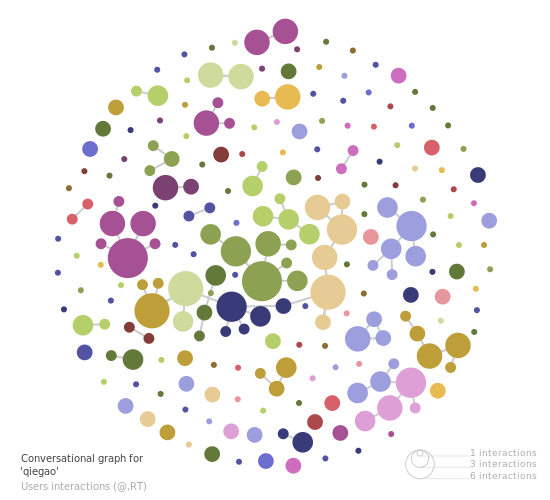
\includegraphics[width=3.0705in,height=2.7913in]{figures/chap4/chapitre4-img9.png}
      \label{fig:users-qiegao}
    }
    \subfloat[Dufu]{
      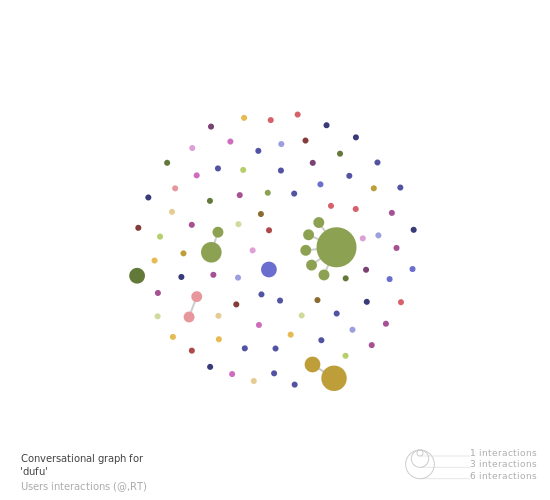
\includegraphics[width=3.0748in,height=2.7913in]{figures/chap4/chapitre4-img10.png}
      \label{fig:users-dufu}
    }
    
  \caption{  
    Graphe conversationnel pour quatre mèmes (sur une durée de 3 semaines)
  }
\end{figure}
% \clearpage

Les graphes de conversation permettent d{\textquoteright}identifier des spécificités et de lire plusieurs indicateurs. Ils rendent notamment bien compte de la taille des conversations, très variables, ou plut\^ot de la dimension des interactions. On voit que les discussions autour d{\textquoteright}aspects politiques et sociétaux suscitent beaucoup plus d{\textquoteright}échanges, alors que les deux autres semblent moins importantes. Dans le cas de \textit{The Voice} (Fig. \ref{fig:users-voice}), la conversation est très structurée autour de peu d{\textquoteright}acteurs qui centralisent les débats. Le mème absurdiste \textit{dufu} (fig. \ref{fig:users-dufu}) est lui composé d{\textquoteright}utilisateurs très distants qui ne communiquent entre eux que faiblement ou par petits groupes. La conversation \textit{sextape }autour du fait divers politique se constitue en groupes structurés mais plus distants. Repoussés vers les bords du graphe, l{\textquoteright}existence de nombreux foyers de discussions montre bien que la discussion a été canalisée autour de groupes spécifiques. A l{\textquoteright}inverse, la discussion de société \textit{qiegao} autour des peuples du Xinjiang (fig. \ref{fig:users-qiegao}) semble se constituer en un vaste foyer de discussions o\`u viennent s{\textquoteright}agréger de nombreux utilisateurs très actifs. 

\subsection[Structures sémantiques]{Structures sémantiques}

La dimension lexicale des contenus web présente une autre approche intéressante \`a explorer pour mieux comprendre comment se structure l{\textquoteright}activité lors de la diffusion des mèmes. La représentation classique du nuage de mots s{\textquoteright}intéresse principalement \`a la quantité de mots en laissant toutefois de coté la mise en relations des mots, pourtant fondamentale dans l{\textquoteright}activité symbolique et expressive. Ainsi, nous avons plut\^ot choisi de donner à voir les réseaux de mots pour comprendre la construction de sens autour de signes particuliers. 

Les relations entre les mots représentent leurs co-occurences dans un même message. La proximité des mots lors des discussions est matérialisée par un graphe disposant les mots par groupe grâce à un algorithme de force. La taille des mots indique le nombre fois qu'ils ont été cités dans les conversations. Les couleurs représentent les communautés détectées par l'algorithme de Louvain \citep{Blondel2008} (voir section \ref{sec:viz} pour plus de détails). Les corpus analysés ici ont été constitués grâce \`a une recherche par mots-clés dans un moteur d{\textquoteright}indexation. Ainsi, les mots les plus proéminents sont bien souvent \`a l{\textquoteright}origine de la constitution du corpus (les mots-clés de la requête utilisée). Ce biais important est \`a prendre en compte dans la lecture de ces graphes.

\begin{figure}[h!]
    \centering
    \subfloat[Dufu]{
      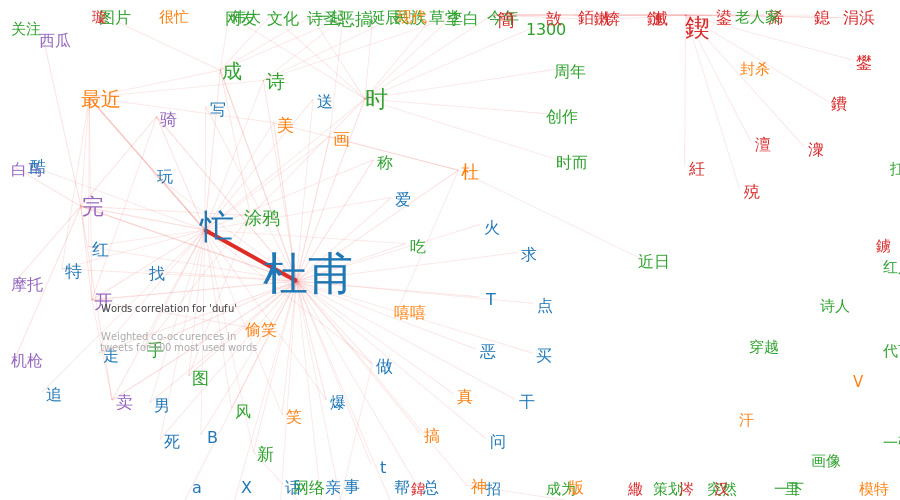
\includegraphics[width=3.1661in,height=1.7594in]{figures/chap4/chapitre4-img11.png}
      \label{fig:words-dufu}
    }
    \subfloat[Yuanfang]{
      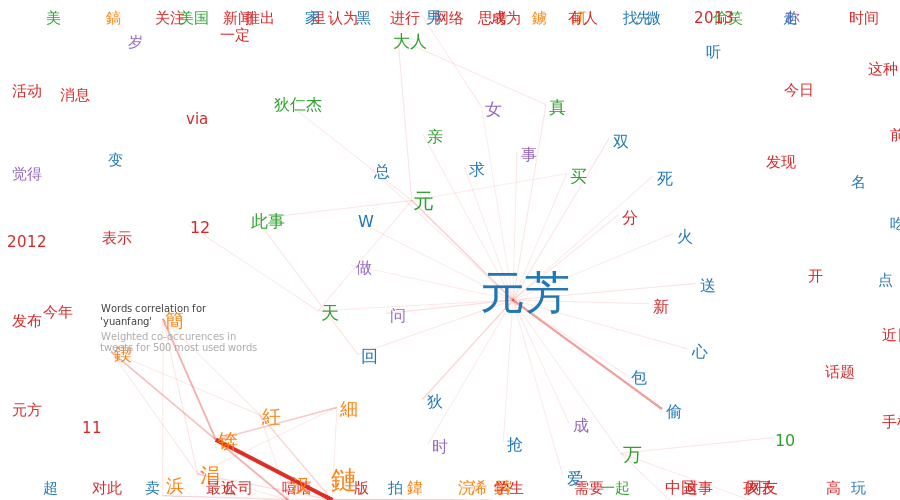
\includegraphics[width=3.1835in,height=1.7697in]{figures/chap4/chapitre4-img12.png}
      \label{fig:words-yuanfang}
    }
    
  \caption{
    Graphe sémantique de co-occurences des mots pour les mèmes dufu et yuanfang   
  }
\end{figure}

En regardant ces figures, nous constatons tout d{\textquoteright}abord que les graphe des mèmes absurdistes (fig. \ref{fig:words-dufu} \& \ref{fig:words-yuanfang}) se compose de peu de mots centraux très fortement connectés et entourés d{\textquoteright}une myriade de mots de faible densité. Ces mots de faible importance correspondent aux multiples déclinaisons qui entrent en jeu dans l'appropriation du mème par jeux de mots.

\begin{figure}[h!]
    \centering
    \subfloat[Sextape]{
      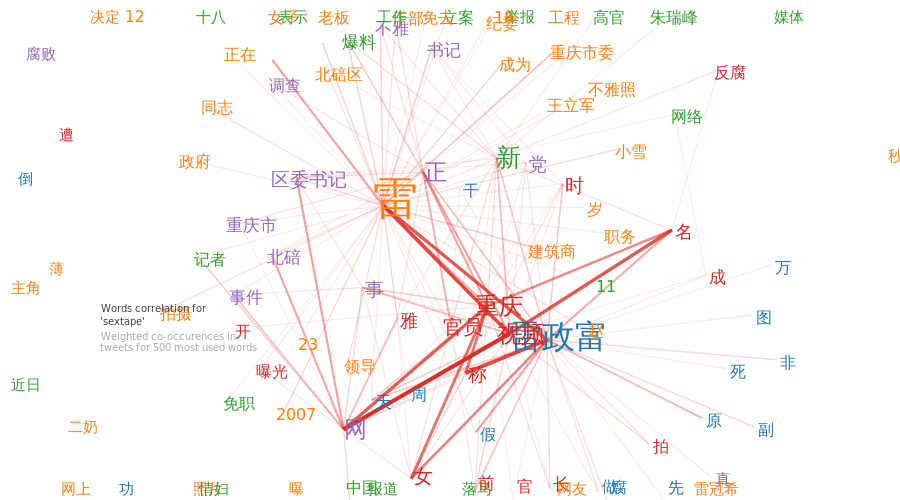
\includegraphics[width=3.1461in,height=1.7504in]{figures/chap4/chapitre4-img13.png}
      \label{fig:words-sextape}
    }
    \subfloat[biaoge]{
      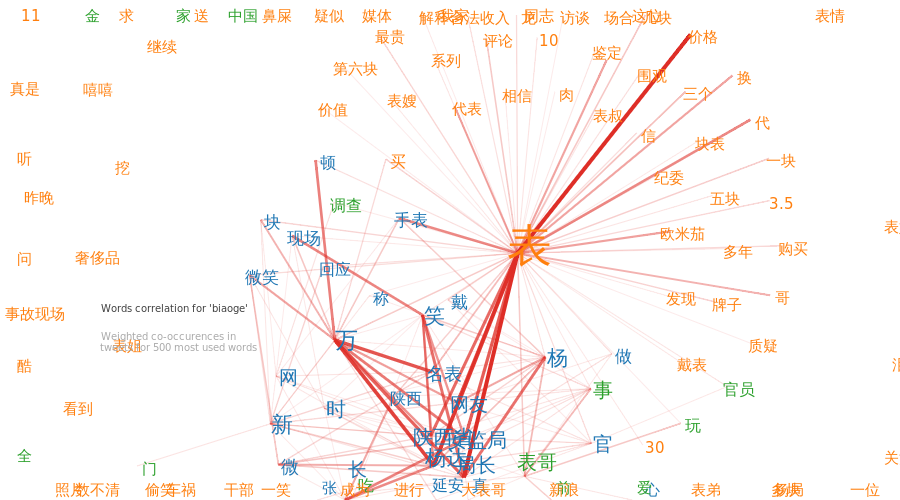
\includegraphics[width=3.2335in,height=1.7961in]{figures/chap4/chapitre4-img14.png}
      \label{fig:words-biaoge}
    }
    
  \caption{
    Graphe sémantique de co-occurences des mots pour les mèmes Sextape et Biaoge
  }
\end{figure}

Les réseaux sémantiques de la discussion concernant les faits divers politiques (fig. \ref{fig:words-sextape} \& \ref{fig:words-biaoge}) sont plus structurés. Ils sont organisés en communautés de mots et de sens plut\^ot bien définies : une communauté décrit les détails de l{\textquoteright}affaire (noms de lieux et de personnes, verbes d{\textquoteright}actions), l{\textquoteright}autre se compose d{\textquoteright}adjectifs discutant le caractère houleux de ces histoires, la dernière est faite de mots plus anecdotiques.

\begin{figure}[h!]
    \centering
    \subfloat[ccp]{
      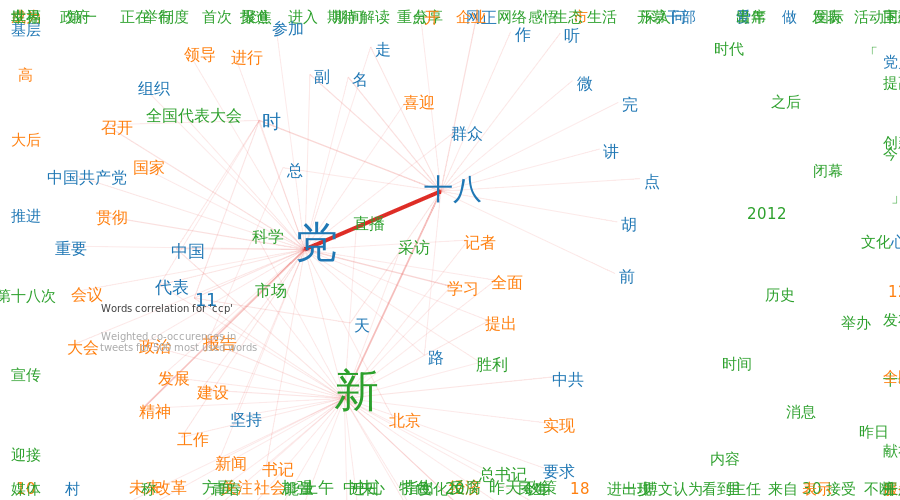
\includegraphics[width=3.0843in,height=1.7134in]{figures/chap4/chapitre4-img15.png}
      \label{fig:words-ccp}
    }
    \subfloat[The Voice]{
      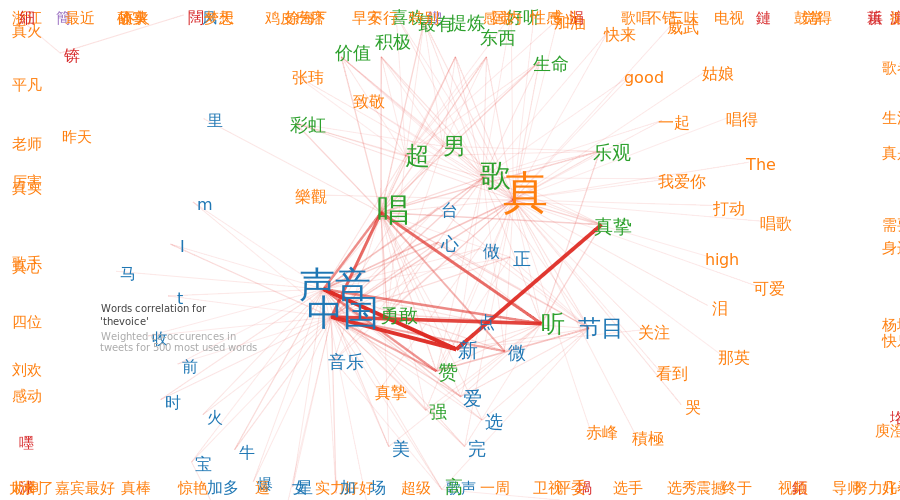
\includegraphics[width=3.0752in,height=1.7122in]{figures/chap4/chapitre4-img16.png}
      \label{fig:words-voice}
    }
    
  \caption{
    Graphe sémantique de co-occurences des mots pour les mèmes CCP et The Voice
  }
\end{figure}

 La structure lexicale qui entoure \textit{The Voice }et \textit{CCP }semble très architecturée, avec des associations plus convenues. Pour \textit{The Voice} (fig. \ref{fig:words-voice}), nous sommes sans surprise en présence du champ lexical du chant (voix-chant, chant-chanson...) entouré par de nombreuses émotions et sentiments (arc-en-ciel-amour, trac-courage, etc.). Nous voyons également que de très nombreux mots ont été propulsés sur les bords du graphe car peu reliés entre eux ou avec le reste du réseau. Reconnus algorithmiquement comme une seule communauté, on y trouve notamment le vocabulaire propre de l{\textquoteright}émission qui ne s'intègre pas au reste des discussions. 

Dans le cas du congrès du parti communiste chinois (fig. \ref{fig:words-ccp}), on retrouve également cette organisation sémantique très hiérarchique autour du mot central {\textquotedblleft}parti{\textquotedblright}, avec un ensemble de signifiants issus du programme politique (construction, développement, loi, science, etc.). Un autre élément prédominent s{\textquoteright}articule autour du caractère {\textquotedblleft}nouveau{\textquotedblright} (révolution, changement, futur...). Comme dans le cas de \textit{The Voice}, nous sommes en présence d{\textquoteright}un langage stéréotypé qui donne lieu \`a un graphe très structuré selon des axes de communication définis. Proportionnellement, une grande partie des discussions est située aux frontières du graphe, très peu reliée avec le reste de l{\textquoteright}activité.

\begin{figure}[h!]
    \centering
    \subfloat[qiegao]{
      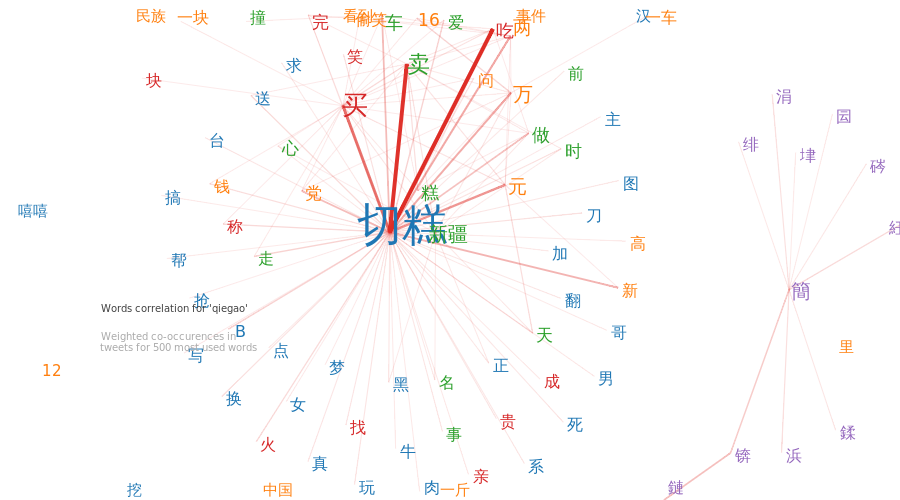
\includegraphics[width=2.9248in,height=1.6252in]{figures/chap4/chapitre4-img17.png}
      \label{fig:words-qiegao}
    }
    \subfloat[moyan]{
      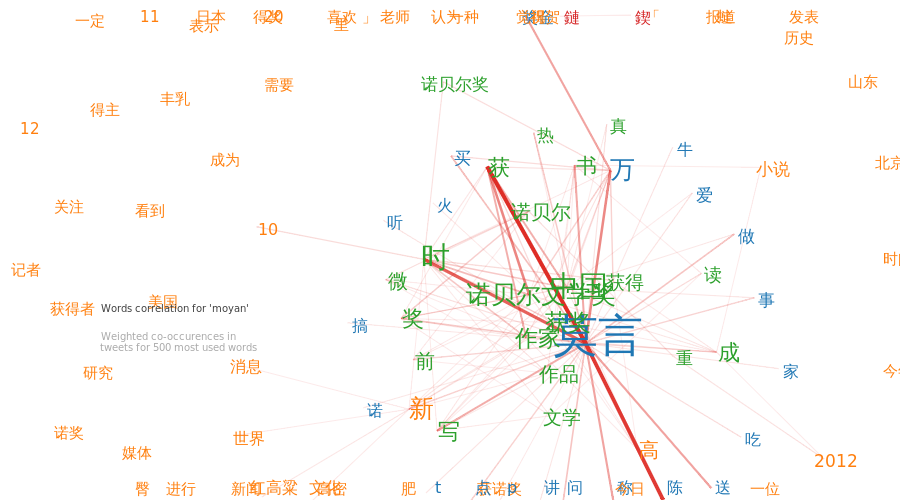
\includegraphics[width=2.978in,height=1.6551in]{figures/chap4/chapitre4-img18.png}
      \label{fig:words-moyan} 
    }
    
  \caption{
    Graphe sémantique de co-occurences des mots pour les mèmes Qiegao et Moyan
  }
\end{figure}


\textit{Qiegao} (fig. \ref{fig:words-qiegao}), quant \`a lui, possède une structure très centralisée articulée autour d{\textquoteright}un mot-clé précis qui relie plusieurs groupes sémantiques (communautés de mots par couleurs) autour de lui. On retrouve cette caractéristique d{\textquoteright}ensemble dans le graphe de \textit{moyan} (fig. \ref{fig:words-moyan}) même si la structuration des communautés sémantiques est plus accentuée. La hiérarchie émergente du graphe montre des mots-clés qui orientent la discussion. Ici, les associations sont plus librement définies mais suivent des champs sémantiques distincts.


\subsection[Dynamiques géographiques et discussions entre provinces]{Dynamiques géographiques et discussions entre provinces}

Nous avons proposé dans cette recherche le terme de milieu numérique afin notamment de problématiser les rapports existants entre les pratiques de la discussion en ligne sur \textit{Sina Weibo} et l{\textquotesingle}espace de la Chine urbaine moderne. Afin de poursuivre notre interrogation, nous allons désormais observer comment les topologies de diffusion en ligne peuvent se corréler avec la réalité géographique. La diffusion d{\textquotesingle}un mème suit-elle la hiérarchie urbaine classique ou bien la géographie urbaine de l{\textquotesingle}Internet? Existe-t-il des modèles de diffusion selon les types de contenus? Quels sont les \textit{patterns }géographiques décrits pas la circulation des contenus? 

Pour tenter de répondre \`a ces différentes questions, nous disposons de données concernant les provinces d{\textquoteright}origine des utilisateurs grâce à leurs informations de profil de Sina Weibo. Une première analyse de la diffusion géographique des mèmes se fera par la projection sur des cartes des échanges entre les utilisateurs. La province d'origine est assigné à chacun des membres des réseaux conversationnels précédemment identifié afin de représenter la dynamique des échanges. Les dynamiques mineures de contenus apparaissent car le volume d'information pour chaque province est pondérée par sa présence dans l'échantillon de la population totale. L{\textquoteright}épaisseur des traits exprime le volume des échanges en pourcentage du total sur la période observée.

\begin{figure}[h!]
  \begin{minipage}[c]{.45\linewidth}
    \centering
    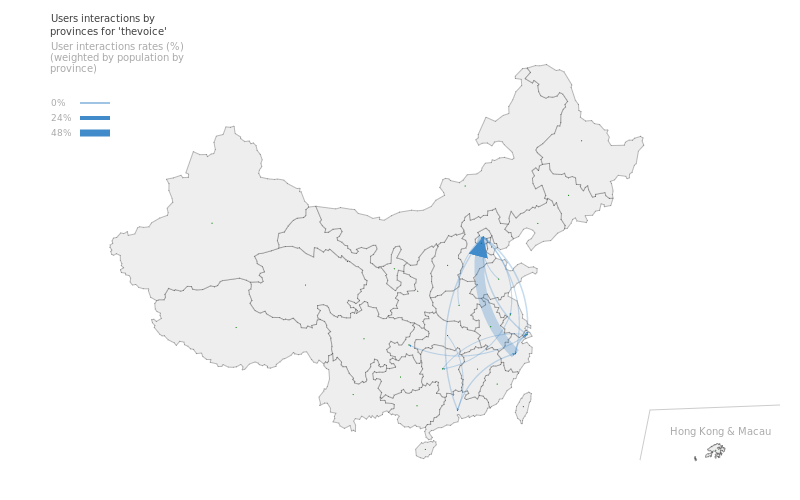
\includegraphics[scale=.3]{figures/chap4/chapitre4-img19.png}
    \caption{
      The Voice: Interaction des utilisateurs par province entre le 9 et le 29 Juillet 2012
    }
    \label{fig:geo-voice-t1}
  \end{minipage}
  \begin{minipage}[c]{.45\linewidth}
    \centering
    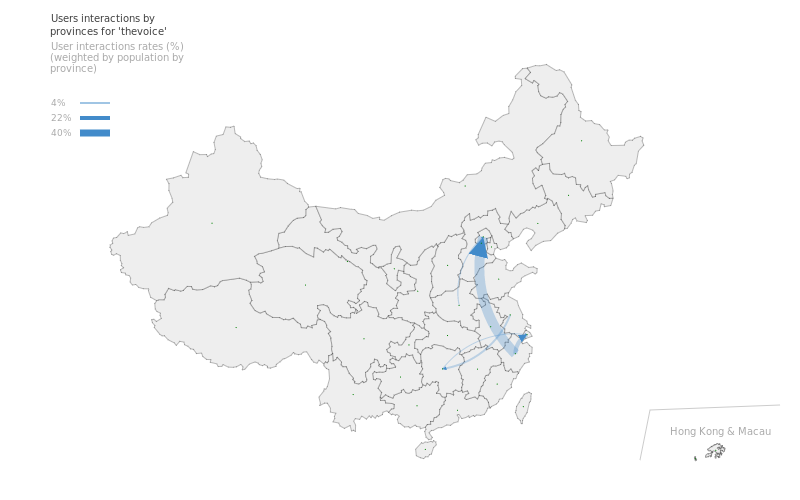
\includegraphics[scale=.3]{figures/chap4/chapitre4-img20.png}    
    \caption{
      The Voice: Interaction des utilisateurs par province entre le 16 et le 17 Juillet 2012
    }
    \label{fig:geo-voice-t2}
  \end{minipage}
\end{figure}

Dans le cas de \textit{The Voice} (fig. \ref{fig:geo-voice-t1}), nous pouvons voir que l{\textquoteright}interaction est structurée autour d{\textquoteright}un axe fort entre la province de Zhejiang et Pékin. Cela s{\textquoteright}explique assez simplement par le fait que l{\textquoteright}émission est diffusée par \textit{Zhejiang TV} dont le compte officiel joue un r\^ole important dans la diffusion et la promotion de la discussion. En isolant uniquement le soir de la première diffusion (fig. \ref{fig:geo-voice-t2}), on voit que cette structure s{\textquoteright}accentue encore davantage. Les interactions se structurent alors entre le Zhejiang, Pékin et Shanghai ainsi que quelques axes plus minoritaires.

\begin{figure}[h!]
    \centering
    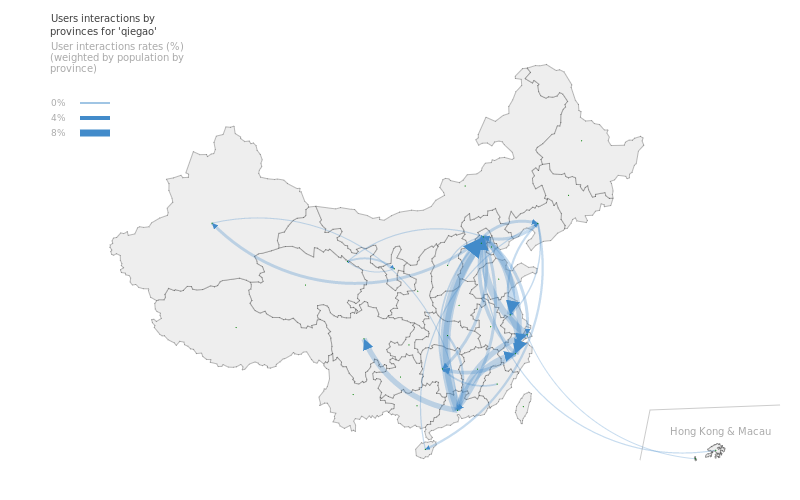
\includegraphics[scale=.35]{figures/chap4/chapitre4-img21.png}
    \caption{
      Qiegao: Interaction des utilisateurs par province entre le 19 Novembre et le 15 Décembre 2012
    }
    \label{fig:geo-qiegao-t0}
\end{figure}

A l{\textquoteright}inverse, nous voyons que pour \textit{Qiegao} (fig. \ref{fig:geo-qiegao-t0}) les patterns semblent beaucoup plus diversifiés. Guangzhou joue un r\^ole de diffuseur important et beaucoup d{\textquoteright}informations converge vers Shanghai et Pékin. De nombreuses conversations se déroulent également dans l{\textquoteright}ouest de la Chine. En effet, la discussion concerne ici les peuples Uyghur et on constate que les habitants du Xinjiang participent davantage \`a la conversation que dans d{\textquoteright}autres mèmes.  

\begin{figure}[h!]
    \centering
    \subfloat[J1: 3 Décembre 2012]{
      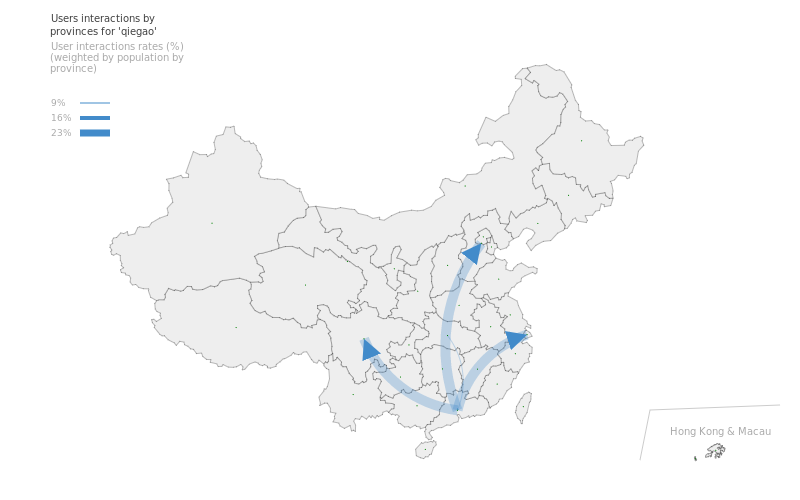
\includegraphics[width=2in,height=1.61in]{figures/chap4/chapitre4-img22.png}
      \label{fig:geo-qiegao-t1}
    }
    \subfloat[J2-3: 4-5 Décembre 2012]{
      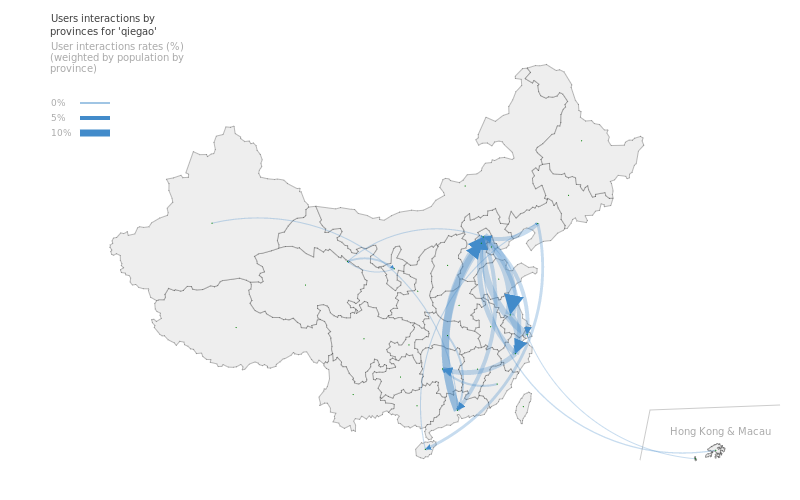
\includegraphics[width=2in,height=1.61in]{figures/chap4/chapitre4-img23.png} 
      \label{fig:geo-qiegao-t2}   
    }
    \newline
    \subfloat[J4-6: 6-8 Décembre 2012]{
      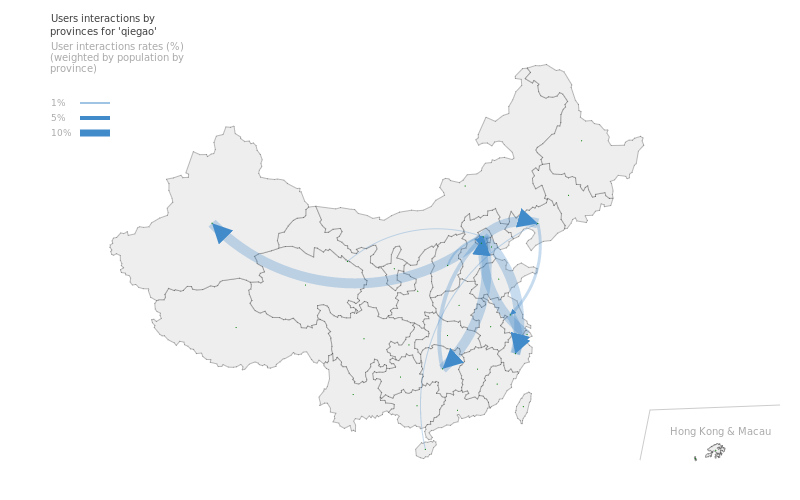
\includegraphics[width=2in,height=1.61in]{figures/chap4/chapitre4-img24.png}
      \label{fig:geo-qiegao-t3}
    }
    \subfloat[J7+: 9-16 Décembre 2012]{
      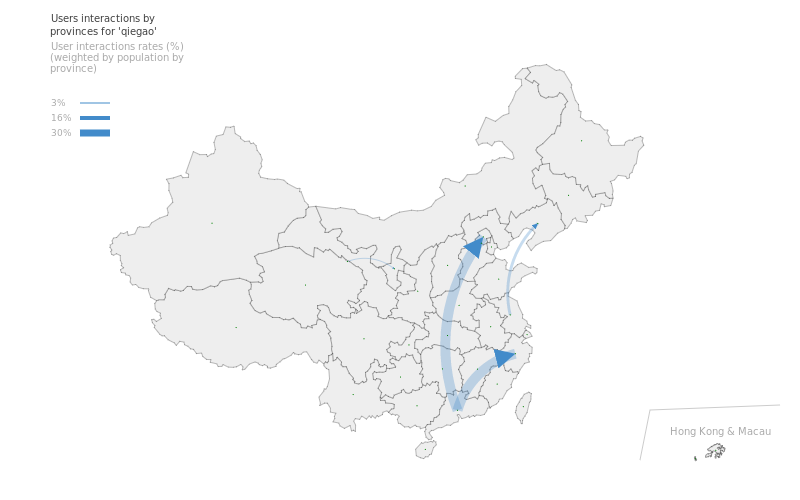
\includegraphics[width=2.8724in,height=1.7961in]{figures/chap4/chapitre4-img25.png}  
      \label{fig:geo-qiegao-t4}
  
    }
    
  \caption{
    Qiegao: Interaction des utilisateurs par province
  }
\end{figure}

En considérant l{\textquoteright}évolution de \textit{qiegao} dans le temps, nous voyons qu{\textquoteright}il émane d{\textquoteright}abord de Canton (fig. \ref{fig:geo-qiegao-t1}), puis se diffuse \`a Pékin et Shanghai (fig. \ref{fig:geo-qiegao-t2}) qui semble jouer un r\^ole d{\textquoteright}amplificateur en le diffusant plus largement (fig. \ref{fig:geo-qiegao-t4}), notamment vers l{\textquoteright}Ouest (fig. \ref{fig:geo-qiegao-t3}).  

\begin{figure}[h!]
    \centering
    
    \subfloat[J1: 22 Novembre 2012]{
      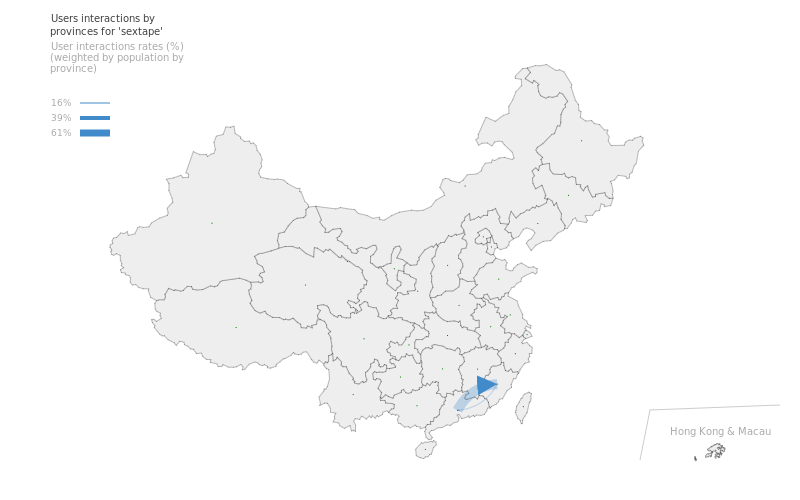
\includegraphics[width=1.9587in,height=1.2248in]{figures/chap4/chapitre4-img26.png}
      \label{fig:geo-sextape-t1}
    }
    \subfloat[J2-5: 23-25 Novembre 2012]{
      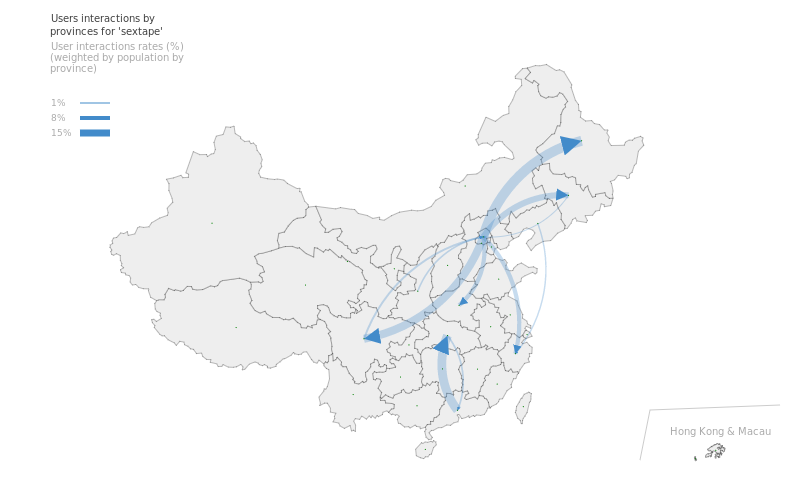
\includegraphics[width=1.9386in,height=1.2114in]{figures/chap4/chapitre4-img27.png}
      \label{fig:geo-sextape-t2}
    }
    \subfloat[J5+: 26 Nov-15 Déc 2012]{
      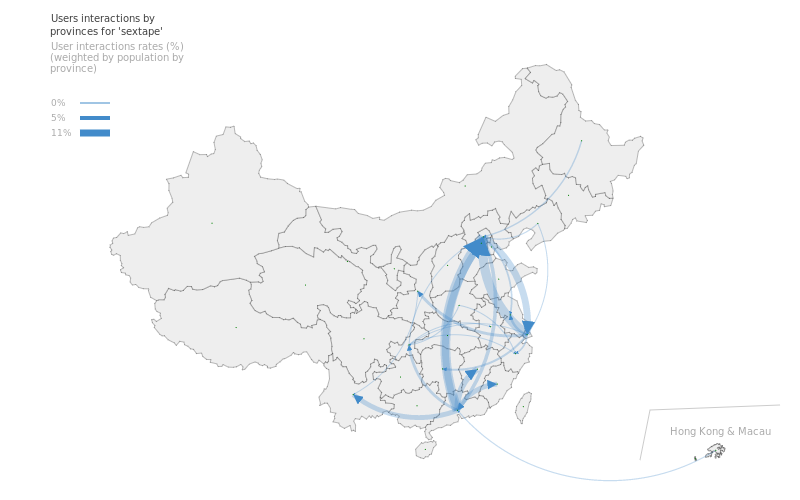
\includegraphics[width=2.0012in,height=1.2512in]{figures/chap4/chapitre4-img28.png}
      \label{fig:geo-sextape-t3}
    }    
  \caption{
    Sextape: Interaction des utilisateurs par province
  }
\end{figure}

On retrouve également ce pattern pour d{\textquoteright}autres faits de société comme \textit{sextape} ou \textit{biaoge}. Cela illustre bien le r\^ole particulier des médias du sud de la Chine et plus spécialement celui de Guangzhou (fig. \ref{fig:geo-sextape-t1} \& \ref{fig:geo-biaoge-t1}).

\begin{figure}[h!]
    \subfloat[J1-3 : 26-28 Aout 2012 ]{
      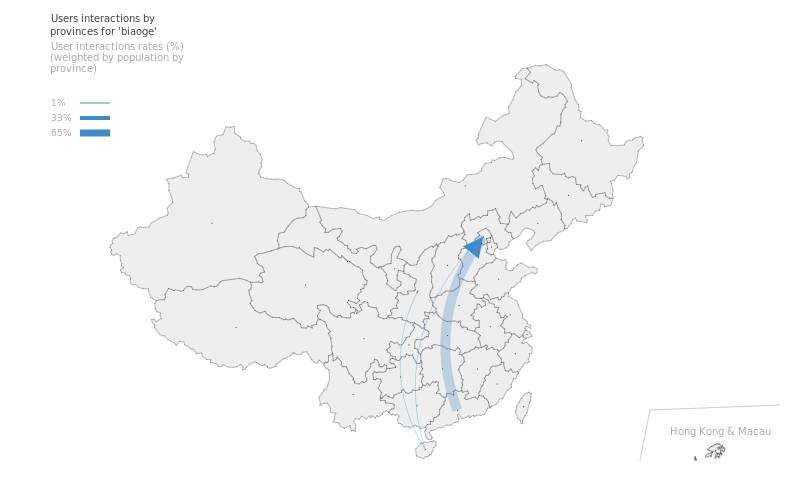
\includegraphics[width=1.9004in,height=1.1878in]{figures/chap4/chapitre4-img29.png}
      \label{fig:geo-biaoge-t1}
    }
    \subfloat[J4-5 : 29-30 Aout 2012 ]{
      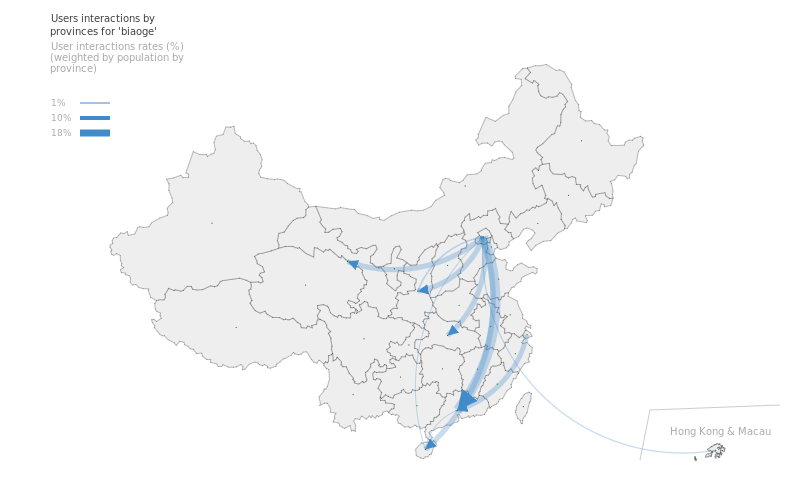
\includegraphics[width=1.9004in,height=1.1878in]{figures/chap4/chapitre4-img30.png} 
      \label{fig:geo-biaoge-t2}
    }
    \subfloat[J5+ : 1-3 Septembre2012]{
      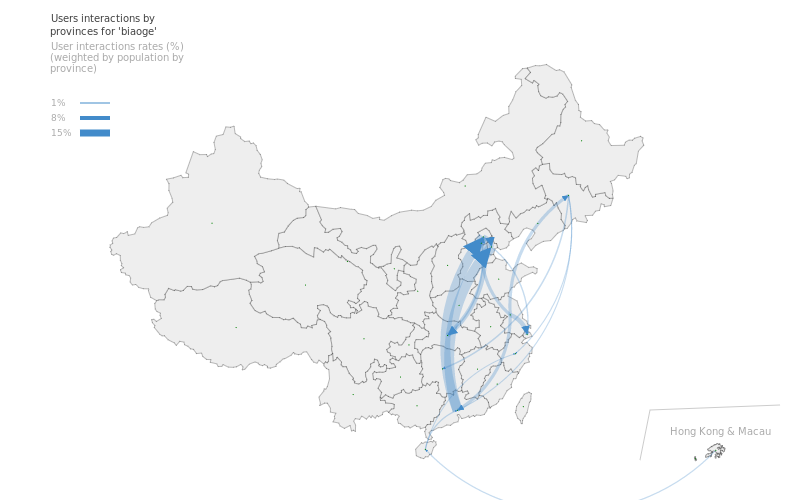
\includegraphics[width=1.9004in,height=1.1878in]{figures/chap4/chapitre4-img31.png} 
      \label{fig:geo-biaoge-t3}
    }
  \caption{
    Biaoge: Interaction des utilisateurs par province
  }
\end{figure}

Avec une plus grande liberté de ton et une plus grande latitude dans leur propos, les médias cantonais sont bien souvent instigateurs d{\textquoteright}affaires importantes alors que les médias pékinois, plus conservateurs joue plut\^ot un r\^ole de diffuseur.  

\begin{figure}[h!]
    \subfloat[ Qiegao]{
      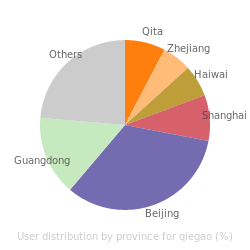
\includegraphics[width=1.9016in,height=1.9016in]{figures/chap4/chapitre4-img33.png}
    }
    \subfloat[Sextape]{
      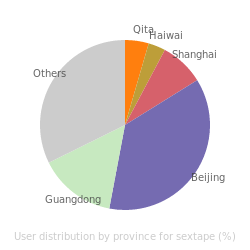
\includegraphics[width=1.9016in,height=1.9016in]{figures/chap4/chapitre4-img34.png}
    }
    \subfloat[Biaoge]{
      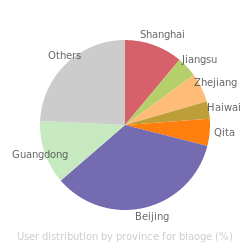
\includegraphics[width=1.9016in,height=1.9016in]{figures/chap4/chapitre4-img35.png}
    }
  \caption{
    Répartition des utilisateurs par province (en \% du total)
    \label{fig:users-share}
  }
\end{figure}


En observant la répartition des utilisateurs par province pour chacun de ces trois mèmes (fig. \ref{fig:users-share}), on remarque que Beijing, Canton, Shanghai ont une place importante, ainsi que les personnes situées \`a l{\textquoteright}étranger (Haiwai) et le Zhejiang. Néanmoins, le reste des provinces (représentés ici par {\textquotedblleft}Others{\textquotedblright} en gris) constitue une part importante des échanges.

\begin{figure}[h!]
    \centering
    \subfloat[J1: 12 Octobre 2012]{
      \label{fig:geo-moyan-t1}
      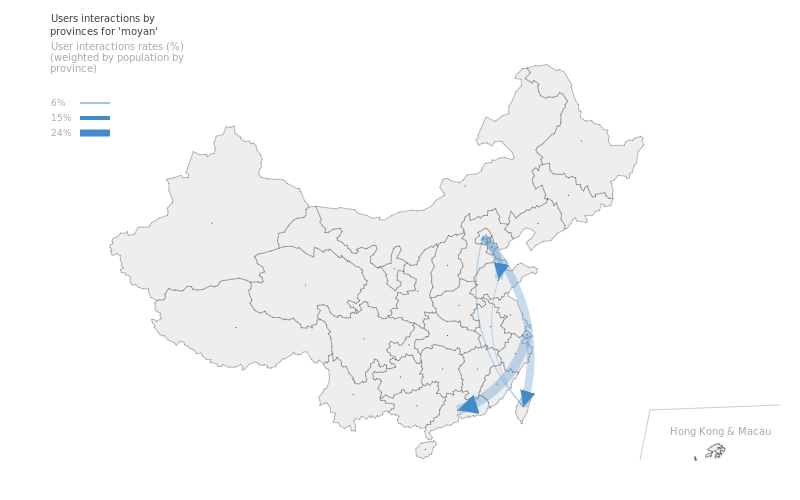
\includegraphics[width=1.9004in,height=1.1878in]{figures/chap4/chapitre4-img36.png}
    }
    \subfloat[J2: 13 Octobre 2012]{
      \label{fig:geo-moyan-t2}
      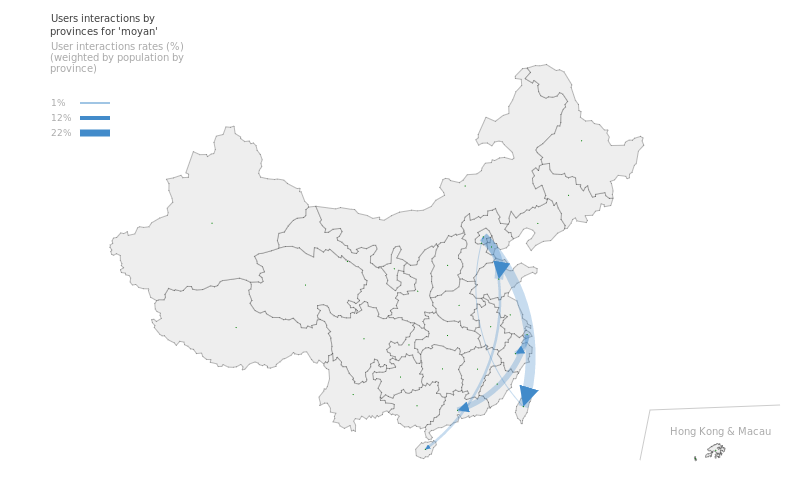
\includegraphics[width=1.9004in,height=1.1878in]{figures/chap4/chapitre4-img37.png}
    }
    \subfloat[J3+: 14-21 Octobre 2012]{
      \label{fig:geo-moyan-t3}
      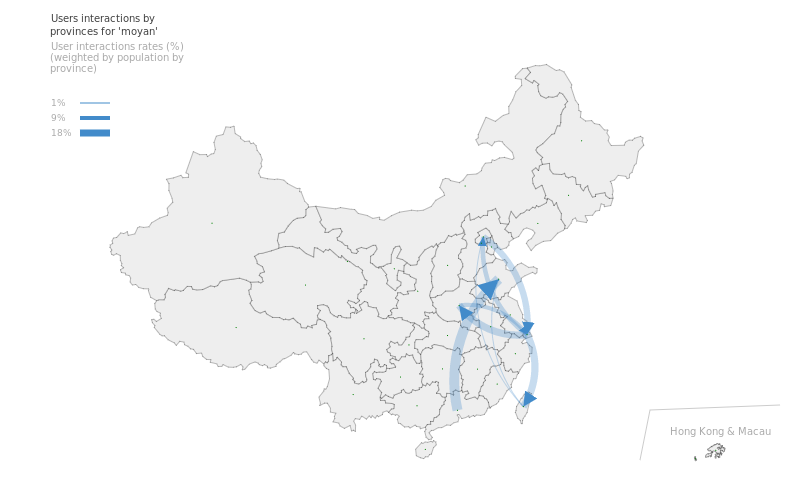
\includegraphics[width=1.9004in,height=1.1878in]{figures/chap4/chapitre4-img38.png}
    }
    \caption{Moyan : Interaction des utilisateurs par province   }
\end{figure}

Dans le cas de nouvelles plus officielles comme pour \textit{Moyan} notamment, nous pouvons voir que l{\textquoteright}information s{\textquoteright}origine généralement de Pékin (fig. \ref{fig:geo-moyan-t1}) et se diffuse vers le sud et le centre (fig. \ref{fig:geo-moyan-t2}). 

\begin{figure}[h!]
    \centering
    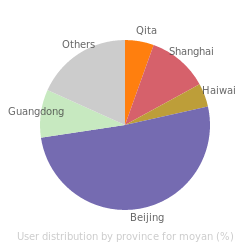
\includegraphics[width=2.6043in,height=2.6043in]{figures/chap4/chapitre4-img39.png}
  \caption{
    Répartition des utilisateurs par province pour Moyan (en \% du total)\\
  }
  \label{fig:geo-moyan-pie}
\end{figure}

La composition des utilisateurs (fig. \ref{fig:geo-moyan-pie}) montre bien que les débats autour de Moyan sont très largement dominés par Pékin avec plus de 50\% de l{\textquoteright}activité impliquant au moins un utilisateur identifié \`a Pékin.

Les mèmes absurdistes et comiques ne semblent pas se construire selon les patterns classiques que nous avons pu observer auparavant.

\begin{figure}[h!]
    \centering
    \subfloat[dufu]{
      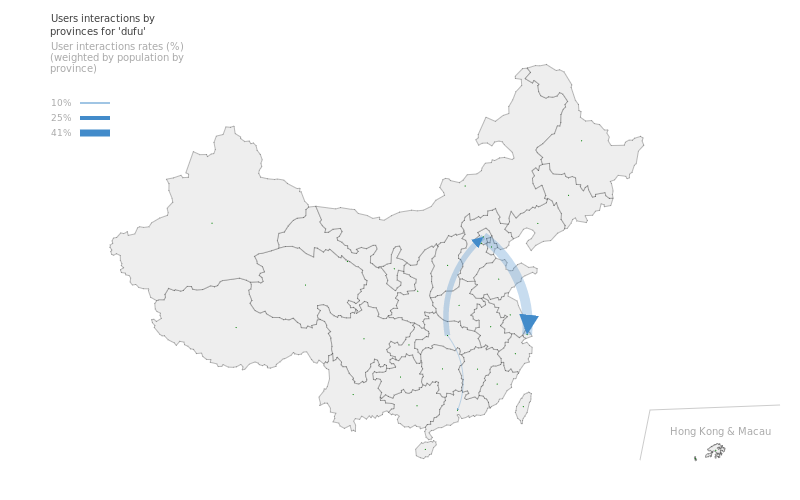
\includegraphics[width=2.9252in,height=1.828in]{figures/chap4/chapitre4-img40.png}
      \label{geo-dufu}
    }
    \subfloat[yuanfang]{ 
      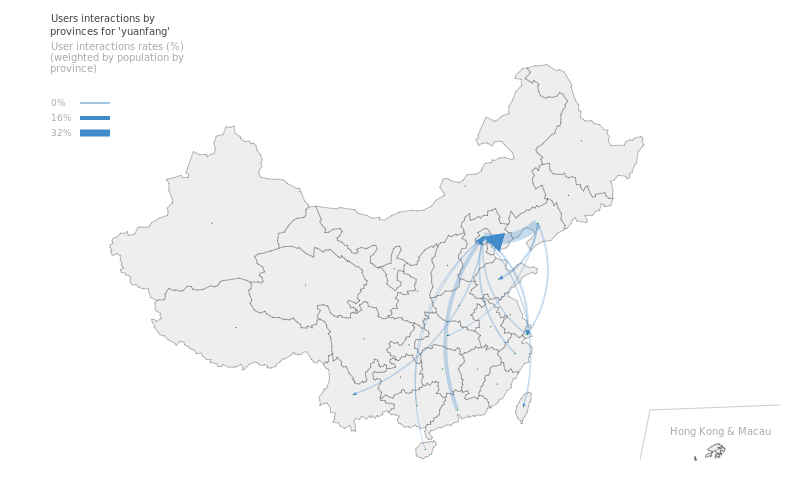
\includegraphics[width=2.9252in,height=1.828in]{figures/chap4/chapitre4-img41.png}
      \label{geo-yuanfang}
    }
    \caption{
        Interaction des utilisateurs par province
    }
\end{figure}


On voit notamment que le mème \textit{dufu } (fig. \ref{geo-dufu}) débute dans la région du Hubei alors que le Liaoning joue un r\^ole clé dans la diffusion de \textit{yuanfang} (fig. \ref{geo-yuanfang}). 

\begin{figure}[h!]
    \centering
    \subfloat[(Dufu) J1-2 : 23 au 25 Mars 2012 ]{
      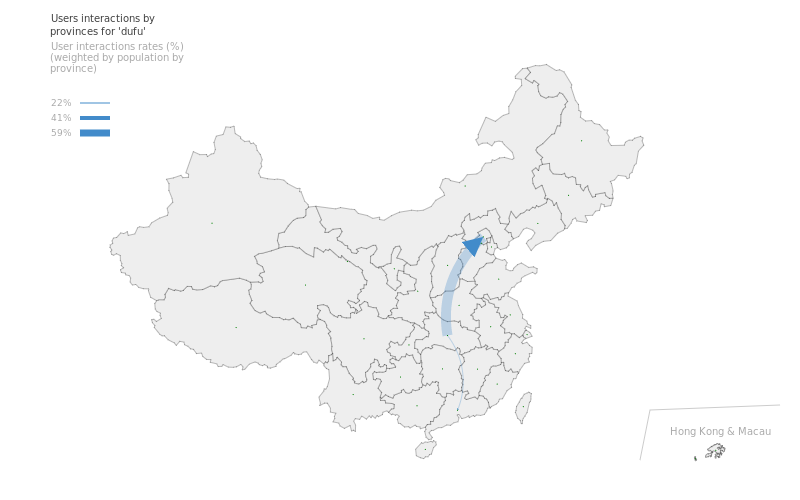
\includegraphics[width=2.9252in,height=1.828in]{figures/chap4/chapitre4-img42.png}
      \label{geo-dufu-t1}
    }
    \subfloat[(Dufu) J3+ : 25 Mars au 15 Avril]{
      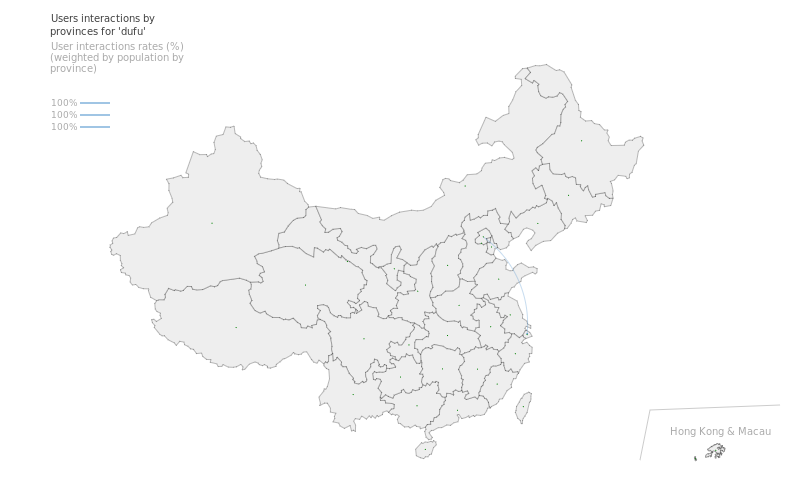
\includegraphics[width=2.9713in,height=1.8571in]{figures/chap4/chapitre4-img43.png}
      \label{geo-dufu-t2}
    }
    \newline
    \subfloat[(Yuanfang) 1-2: 15 au 17 Octobre 2012]{
      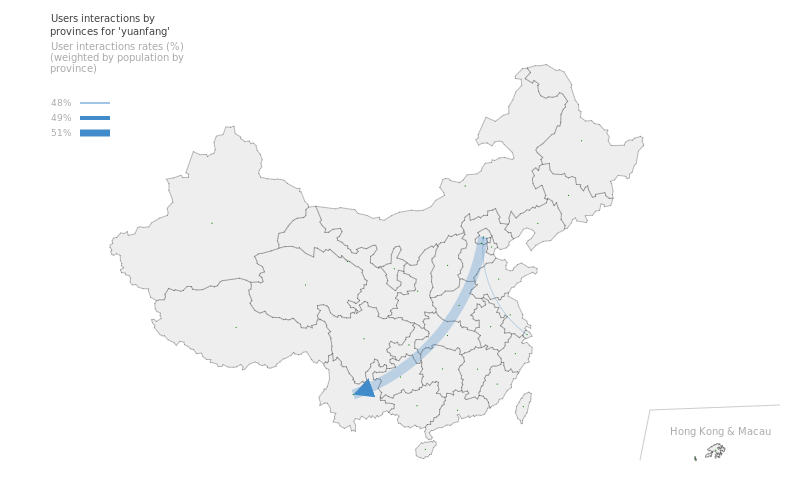
\includegraphics[width=2.9252in,height=1.828in]{figures/chap4/chapitre4-img44.png}
      \label{geo-yuanfang-t1}
    }
    \subfloat[(Yuanfang) J3+: 18 Oct au 16 Décembre 2012]{
      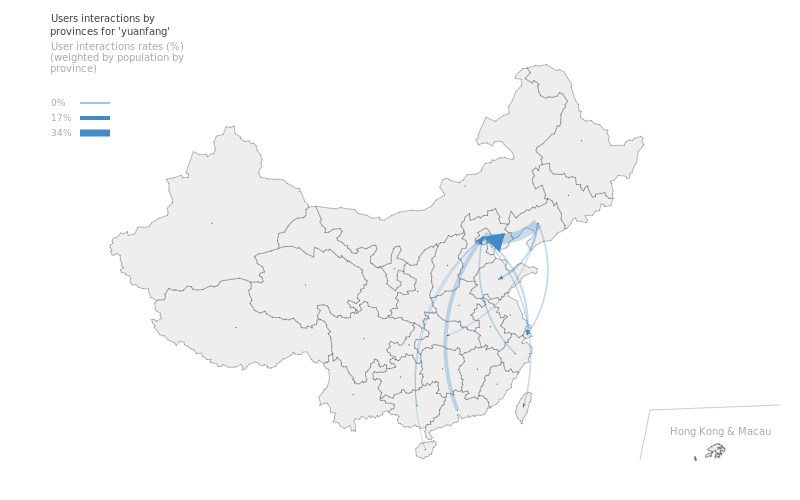
\includegraphics[width=2.9252in,height=1.828in]{figures/chap4/chapitre4-img45.png}
      \label{geo-yuanfang-t2}
    }
    
    \caption{
        Evolution des interactions des utilisateurs par province pour Dufu et Yuanfang
    }
\end{figure}


En considérant les graphes de temps, on remarque également que si Pékin est bien présent, les échanges des premiers jours se font principalement avec le Hubei (fig. \ref{geo-dufu-t1}) et le Yunnan (fig. \ref{geo-yuanfang-t1}), deux provinces typiquement peu actives. Dans un second temps, l'activité se concentre sur les régions cotières (fig. \ref{geo-yuanfang-t2}).

En s{\textquoteright}intéressant aux échanges qui se déroulent au sein de chaque province (d{\textquoteright}un utilisateur situé dans une province vers un autre utilisateur situé dans la même province) (fig. \ref{geo-same-yuanfang} \& \ref{geo-same-dufu}),nous constatons que les échanges internes sont également importants au sein des villes principales (Canton, Pékin et Shanghai).

\begin{figure}[h!]
    \centering
    \subfloat[dufu]{
      \includegraphics[width=2.9252in,height=1.828in]{figures/chap4/chapitre4-img46.png}
      \label{geo-same-dufu}
    }
    \subfloat[yuanfang]{
      \includegraphics[width=2.9252in,height=1.828in]{figures/chap4/chapitre4-img47.png}
      \label{geo-same-yuanfang}
    }
    \caption{
        Interaction entre utilisateurs de la même province
    }
\end{figure}

Néanmoins, de nombreuses villes prennent aussi part \`a la discussion (fig. \ref{geo-pie-yuanfang} \& \ref{geo-pie-dufu}). 


\begin{figure}[h!]
    \centering
    \subfloat[dufu]{
      \includegraphics[scale=0.5]{figures/chap4/chapitre4-img48.png}
      \label{geo-pie-dufu}
    }
    \subfloat[yuanfang]{
      \includegraphics[scale=0.5]{figures/chap4/chapitre4-img49.png}
      \label{geo-pie-yuanfang}
    }
    \caption{
        Répartition des utilisateurs par province (en \% du total)
    }

\end{figure}

La plupart des contenus paraissent suivre des modèles connus, à l'exception des mèmes absurdistes qui présentent des caractéristiques différentes.

\subsection{Communautés, clusters et groupes de provinces}

Un récent article du département d{\textquoteright}urbanisme de l{\textquoteright}Université de Nanjing \citep{Zhen2013} analyse les similarités et différences entre le réseau urbain et le réseau des relations friends/followers entre les utilisateurs sur \textit{Sina Weibo}. Il y est notamment montré que le réseau des relations entre utilisateurs vient renforcer la hiérarchie classique du système urbain. Zhen explique comment Internet vient accélérer l{\textquoteright}agglomération selon des modèles spatiaux pré-existants comme celui des \textit{``Three majors and four smalls''}, accentuant ainsi la différence très marquée entre l{\textquoteright}Ouest et l{\textquoteright}Est de la Chine.

\begin{figure}[h!]
    \centering
    
    \begin{description}
    \item[Three Majors]
        \hfill \\
      \begin{enumerate}
      \item Pearl River Delta (Guangzhou, Shenzhen)
      \item Beijing-Tianjin-Hebei region (Beijing)
      \item the Yangtze River Delta (Shanghai, Hangzhou, Nanjing)
      \end{enumerate}

    \item[Four Smalls]
    \hfill \\
      \begin{enumerate}
      \item Chengdu-Chongqing region (Chengdu, Chongqing)
      \item Hercynian region (Fuzhou, Xiamen)
      \item Wuhan (central) region (Wuhan, Changsha)
      \item Northeast China (Shenyang, Harbin, Changchun)
      \end{enumerate}

    \end{description}

   \caption{
      Le modèle urbain chinois du Three majors and four smalls d{\textquoteright}après \cite{Zhen2013}
    }
\end{figure}

Les résultats obtenus par l'analyse du réseau des followers sur \textit{Sina Weibo} peuvent être comparés avec les phénomènes observés lors de la diffusion de contenus. En effet, si on peut affirmer que le réseau {\textquotedblleft}d{\textquoteright}amis{\textquotedblright} structure les canaux de diffusion de \textit{Sina Weibo}, ces canaux ne sont pas nécessairement sujets \`a une utilisation fréquente et donc \`a l{\textquoteright}actualisation de ces structures. Il peut donc être intéressant d'observer les façons dont ces canaux sont activés lors des conversations en ligne.

Reprenant le réseau des interactions entre provinces constitué par les échanges des utilisateurs, nous souhaitons désormais observer les communautés de discussion se formant entre des provinces spécifiques lors de la diffusion des contenus sur \textit{Sina Weibo}. Nous soumettons donc le réseau d{\textquoteright}interactions entre provinces \`a un algorithme de Louvain \citep{Blondel2008} qui nous permet d'identifier les provinces ayant le plus interagit ensemble. Sur les cartes, les couleurs représentent les différentes communautés calculées depuis le réseau d{\textquoteright}interactions. 

\begin{figure}[h!]
    \centering

    \subfloat[sextape]{
      \includegraphics[width=3.198in,height=2.0004in]{figures/chap4/chapitre4-img50.png}
      \label{geo-clusters-sextape}
    }
    \subfloat[TheVoice]{
      \includegraphics[width=3.3024in,height=2.063in]{figures/chap4/chapitre4-img51.png}
      \label{geo-clusters-voice}
    } 
    \newline
    \subfloat[Qiegao]{
      \includegraphics[width=3.1878in,height=1.9795in]{figures/chap4/chapitre4-img52.png}
      \label{geo-clusters-qiegao}
    } 
    \subfloat[Dufu]{
      \includegraphics[width=3.5315in,height=2.2087in]{figures/chap4/chapitre4-img53.png}
      \label{geo-clusters-dufu}
    }

    \caption{
        Communauté de provinces dessinées par les échanges entre utilisateurs autour de chaque mème (Algorithme de Louvain).
    }

\end{figure}


\'A la première lecture de ces cartes, nous constatons en effet que les provinces de l{\textquoteright}Ouest sont nettement moins engagées que celles de la moitié Est de la Chine. Ce fait reflète la concentration de la population des utilisateurs de Weibo dans les grandes villes en développement de la c\^ote et du centre \citep{Fu2013}. 

Le mème absurdiste \textit{dufu} possède une diffusion plus concentrée (fig. \ref{geo-clusters-dufu}) alors que les discussions politiques semblent regrouper des utilisateurs d{\textquoteright}origines plus diverses (fig. \ref{geo-clusters-sextape} \& \ref{geo-clusters-qiegao}). Nous remarquons également que Taiwan est absente des discussions plus en lien avec la politique et la société de Chine continentale, alors qu{\textquoteright}elle est bien présente dans le cas des mèmes absurdistes et de l{\textquoteright}émission de loisir (fig. \ref{geo-clusters-voice}). Parmi la diversité de formes visibles sur les cartes, peu de pattern sont néanmoins décelables a priori. La circulation des contenus ne semble pas suivre de patterns définis, mais plutôt posséder des modèles différents pour chaque contenu. Il nous est donc impossible de valider ou réfuter le modèle proposé par l'analyse des relations friends / followers par \cite{Zhen2013}. 

\subsection{Dimensions géographiques des graphes socio-sémantiques}

Ces premières observations nous ont montré que s{\textquoteright}il est possible de mieux comprendre les logiques et dynamiques de diffusion des contenus, il est néanmoins plus périlleux de tirer des conclusions définitives sur les dynamiques géographiques de la diffusion sur l{\textquoteright}ensemble d{\textquoteright}un territoire. De plus, nous ne disposons que de très peu d{\textquotesingle}aspects {\textquotedbl}géo-localisés{\textquotedbl} dans ces données (pas de géotag sur chaque message \`a proprement parler). Nous savons également que la province d{\textquoteright}origine du profil ne peut être considérée comme une source absolument fiable. Les utilisateurs sont en effet libres de la remplir selon leur bon vouloir. Face \`a ces diverses réserves, il est important de recentrer l{\textquoteright}étude sur les dimensions plus facilement observables de la diffusion, notamment socio-sémantiques. Le croisement et les corrélations entre mots, utilisateurs et provinces peuvent nous permettre d'explorer des dynamiques entourant les échanges en ligne.

Tout d{\textquoteright}abord, nous nous proposons d{\textquoteright}observer la distribution des provinces d{\textquoteright}origine des communautés d{\textquoteright}utilisateurs les plus importantes. En sélectionnant les communautés les plus centrales pour chaque graphe, nous pouvons mieux comprendre comment se répartissent les {\textquotedblleft}influenceurs{\textquotedblright} sur le territoire pour chacun des mèmes choisis ici.

\begin{figure}[h!]
    \centering
    \includegraphics[width=5.9996in,height=2.5004in]{figures/chap4/chapitre4-img54.png}
    \caption{
        Communauté de provinces dessinées par les échanges entre utilisateurs autour de Sextape
    }
    \label{fig:sextape-users-pie}
\end{figure}

Les communautés formées lors de la discussion autour des mèmes \`a teneur plus politique présentent une grande diversité de provenances. On voit dans le cas de \textit{biaoge} (fig. \ref{fig:biaoge-users-pie}) et \textit{sextape} (fig. \ref{fig:sextape-users-pie}) que de nombreuses provinces sont représentées.

\begin{figure}[h!]
    \centering     
    \includegraphics[width=5.9996in,height=2.5004in]{figures/chap4/chapitre4-img55.png}
    \caption{
        Communauté de provinces dessinées par les échanges entre utilisateurs autour de Biaoge
    }
    \label{fig:biaoge-users-pie}
\end{figure}

\begin{figure}[h!]
    \centering
    \includegraphics[width=5.9996in,height=2.5004in]{figures/chap4/chapitre4-img56.png}
    \caption{
        Communauté de provinces dessinées par les échanges entre utilisateurs autour de The Voice
    }
    \label{fig:voice-users-pie}
\end{figure}

\'A l{\textquoteright}inverse, les communautés d{\textquoteright}utilisateurs les plus impliquées dans \textit{The Voice} (fig. \ref{fig:voice-users-pie}) ou \textit{Moyan} (fig. \ref{fig:voice-users-pie}) sont pour la plupart localisées \`a Beijing. Par rapport \`a la cartographie précédente qui montrait les relations fortes avec le Zhejiang pour \textit{The Voice} (fig. \ref{fig:voice-users-pie}), nous voyons ici que la province est très faiblement représentée dans les communautés majoritaires. 

\begin{figure}[h!]
  \centering
   \includegraphics[width=5.9996in,height=2.5004in]{figures/chap4/chapitre4-img57.png}
    \caption{
        Communauté de provinces dessinées par les échanges entre utilisateurs autour de Moyan
    }
    \label{fig:moyan-users-pie}
\end{figure}

Le mème \textit{dufu} (fig. \ref{fig:dufu-users-pie}) montre quant \`a lui un pattern différent o\`u les communautés sont organisées plus régionalement, avec moins de diversité d{\textquoteright}origine des utilisateurs engagés dans les discussions. Des groupes plutôt perméables se forment autour de différentes régions.

\begin{figure}
    \centering
    \includegraphics[width=5.9996in,height=2.5004in]{figures/chap4/chapitre4-img58.png}
    \caption{
        Communauté de provinces dessinées par les échanges entre utilisateurs autour de Dufu
    }
    \label{fig:dufu-users-pie}
\end{figure}


Une dimension importante du mème absurdiste semble être l{\textquoteright}organisation des conversations en communautés plut\^ot locales (utilisateurs de même province). Une première analyse des communautés les plus centrales dans le graphe de \textit{yuanfang} ne nous permet pas de retrouver ce pattern. Pourtant, en nous intéressant aux communautés de seconde et troisième importance, nous voyons que la plupart se constituent autour de 1 ou 2 provinces seulement.  

Pour continuer notre exploration de l{\textquoteright}existence géographique des relations socio-sémantiques dans nos mèmes, nous allons maintenant nous intéresser \`a une seconde dimension qui est celle de la distribution des mots par province. Nous sélectionnons pour chaque mème les mots les plus centraux du graphe sémantique et décomposons leur usage afin de comprendre la diversité ou l{\textquoteright}unicité de l{\textquoteright}origine des utilisateurs. 

\begin{figure}[h!]
    \centering
    \includegraphics[width=6.0087in,height=3.3386in]{figures/chap4/chapitre4-img59.png}
    \caption{
      biaoge : distribution des citations par provinces pour le mot wan signifiant 10000, une quantité ici quantité d{\textquoteright}argent pour une montre.
    }
    \label{fig:biaoge-words-pie-wan}
\end{figure}
 
\begin{figure}[h!]
  \centering
  \includegraphics[width=6.0087in,height=3.3386in]{figures/chap4/chapitre4-img60.png}
  \caption{
     biaoge : distribution des citations par provinces pour le mot biao (montre)
  }
  \label{fig:biaoge-words-pie-biao}
\end{figure}


Dans le cas du mème \textit{biaoge} (fig. \ref{fig:biaoge-words-pie-biao} \& \ref{fig:biaoge-words-pie-biao}), nous voyons que les mots principaux portent une forte diversité et confirme l{\textquoteright}hypothèse d{\textquoteright}une diffusion géographique plus large de la discussion.

\begin{figure}[h!]
    \centering

    \subfloat[\textit{zhen}, signifiant {\textquotedblleft}vrai{\textquotedblright}]{
      \includegraphics[scale=0.3]{figures/chap4/chapitre4-img61.png}
    }
    \subfloat[\textit{chang}, signifiant {\textquotedblleft}chanter{\textquotedblright}]{
      \includegraphics[scale=0.3]{figures/chap4/chapitre4-img62.png}
    }
    \newline
    \subfloat[\textit{shengyin}, signifiant ``la voix'']{
      \includegraphics[scale=0.5]{figures/chap4/chapitre4-img63.png}
    }
    \caption{
      The Voice : distribution des citations de mots par provinces 
    }
    \label{fig:voice-words-pie}
\end{figure}


\'A l{\textquoteright}inverse, les mots-clés de \textit{The Voice} (fig. \ref{fig:voice-words-pie}) sont nettement dominés par des communautés d{\textquoteright}utilisateurs de Pékin ou du Zhejiang qui semblent réellement fixer les termes de la discussion.


\begin{figure}[h!]
    \centering
    \subfloat[\textit{zuijin}, signifiant {\textquotedblleft}ces derniers temps{\textquotedblright}]{  
      \includegraphics[scale=0.3]{figures/chap4/chapitre4-img65.png}
    }
    \subfloat[\textit{mang}, signifiant {\textquotedblleft}occupé{\textquotedblright}]{  
      \includegraphics[scale=0.3]{figures/chap4/chapitre4-img66.png}
    }
    \newline
    \subfloat[\textit{dufu}, le nom d'un lettré chinois célèbre]{  
      \includegraphics[scale=0.4]{figures/chap4/chapitre4-img64.png}
    }
    \caption{
      Dufu : distribution des citations de mots par provinces 
    }
    \label{fig:dufu-words-pie}
\end{figure}

Dans le cas de dufu, les trois mots les plus importants \textit{dufu}, \textit{zuijin} et \textit{mang} qui forment la phrase-mème ``\textit{dufu est très occupé récemment}'' sont tous très fortement liés \`a la région de Canton (fig. \ref{fig:dufu-words-pie}). Cette information, pas forcément proéminente dans les analyses précédentes, montre que le développement de ce mème est largement le fait d{\textquoteright}utilisateurs de la région de Canton.

\begin{figure}[h!]
    \centering
    \includegraphics[scale=0.3]{figures/chap4/words_pie_qiegao_Nov_19_2012_Dec_16_2012}
    \caption{
      Qiegao : origine géographique des utilisateurs
    }
    \label{fig:qiegao-words-pie}
\end{figure}

La diversité géographique des utilisateurs utilisant le mot \textit{qiegao} (fig. \ref{fig:qiegao-words-pie}) montrent bien la large extension de ce débat à travers la Chine.